%----------------------------------------------------------------
%
%  File    :  thesis-style.tex
%
%  Author  :  Keith Andrews, IICM, TU Graz, Austria
% 
%  Created :  27 May 93
% 
%  Changed :  19 Feb 2004
% 
% styling and technical implementation adopted 2011 by Karl Voit
%----------------------------------------------------------------

%% defined an anvironment for the style Keith used to use:

\chapter{Tests und Ergebnisse}
\label{chap:Ergebnisse}
Im vorangegangen Kapitel \ref{cap:algorithmus} wurde der Algorithmus für die Zuordnung von Aufgaben zu Subjekten beschrieben. Dieses Kapitel zeigt die Ergebnisse des Algorithmus basierend auf den Testfällen \todo{Max} Link um eine Vergleichbarkeit der Algorithmen zu gewährleisten. 

\section{Testergenisse} % (fold)
\label{sec:testergenisse}

{\setstretch{1.0}
\begin{center}
	\begin{longtabu} to \linewidth {@{}p{.05\linewidth}m{.2\linewidth}p{.1\linewidth}m{.5\linewidth}@{}} 
		\textbf{Nr.} & \textbf{Bild} & \textbf{erkannt} & \textbf{Beschreibung}\\ \midrule \endfirsthead
		\textbf{Nr.} & \textbf{Bild} & \textbf{erkannt} & \textbf{Beschreibung}\\ \midrule \endhead
		\multicolumn{4}{c}{Fortsetzung auf nächster Seite}
		\endfoot
 	   	\caption{Algorithmus - Plausibilität prüfen\label{tab:results}}
 	   	\endlastfoot
		1 & 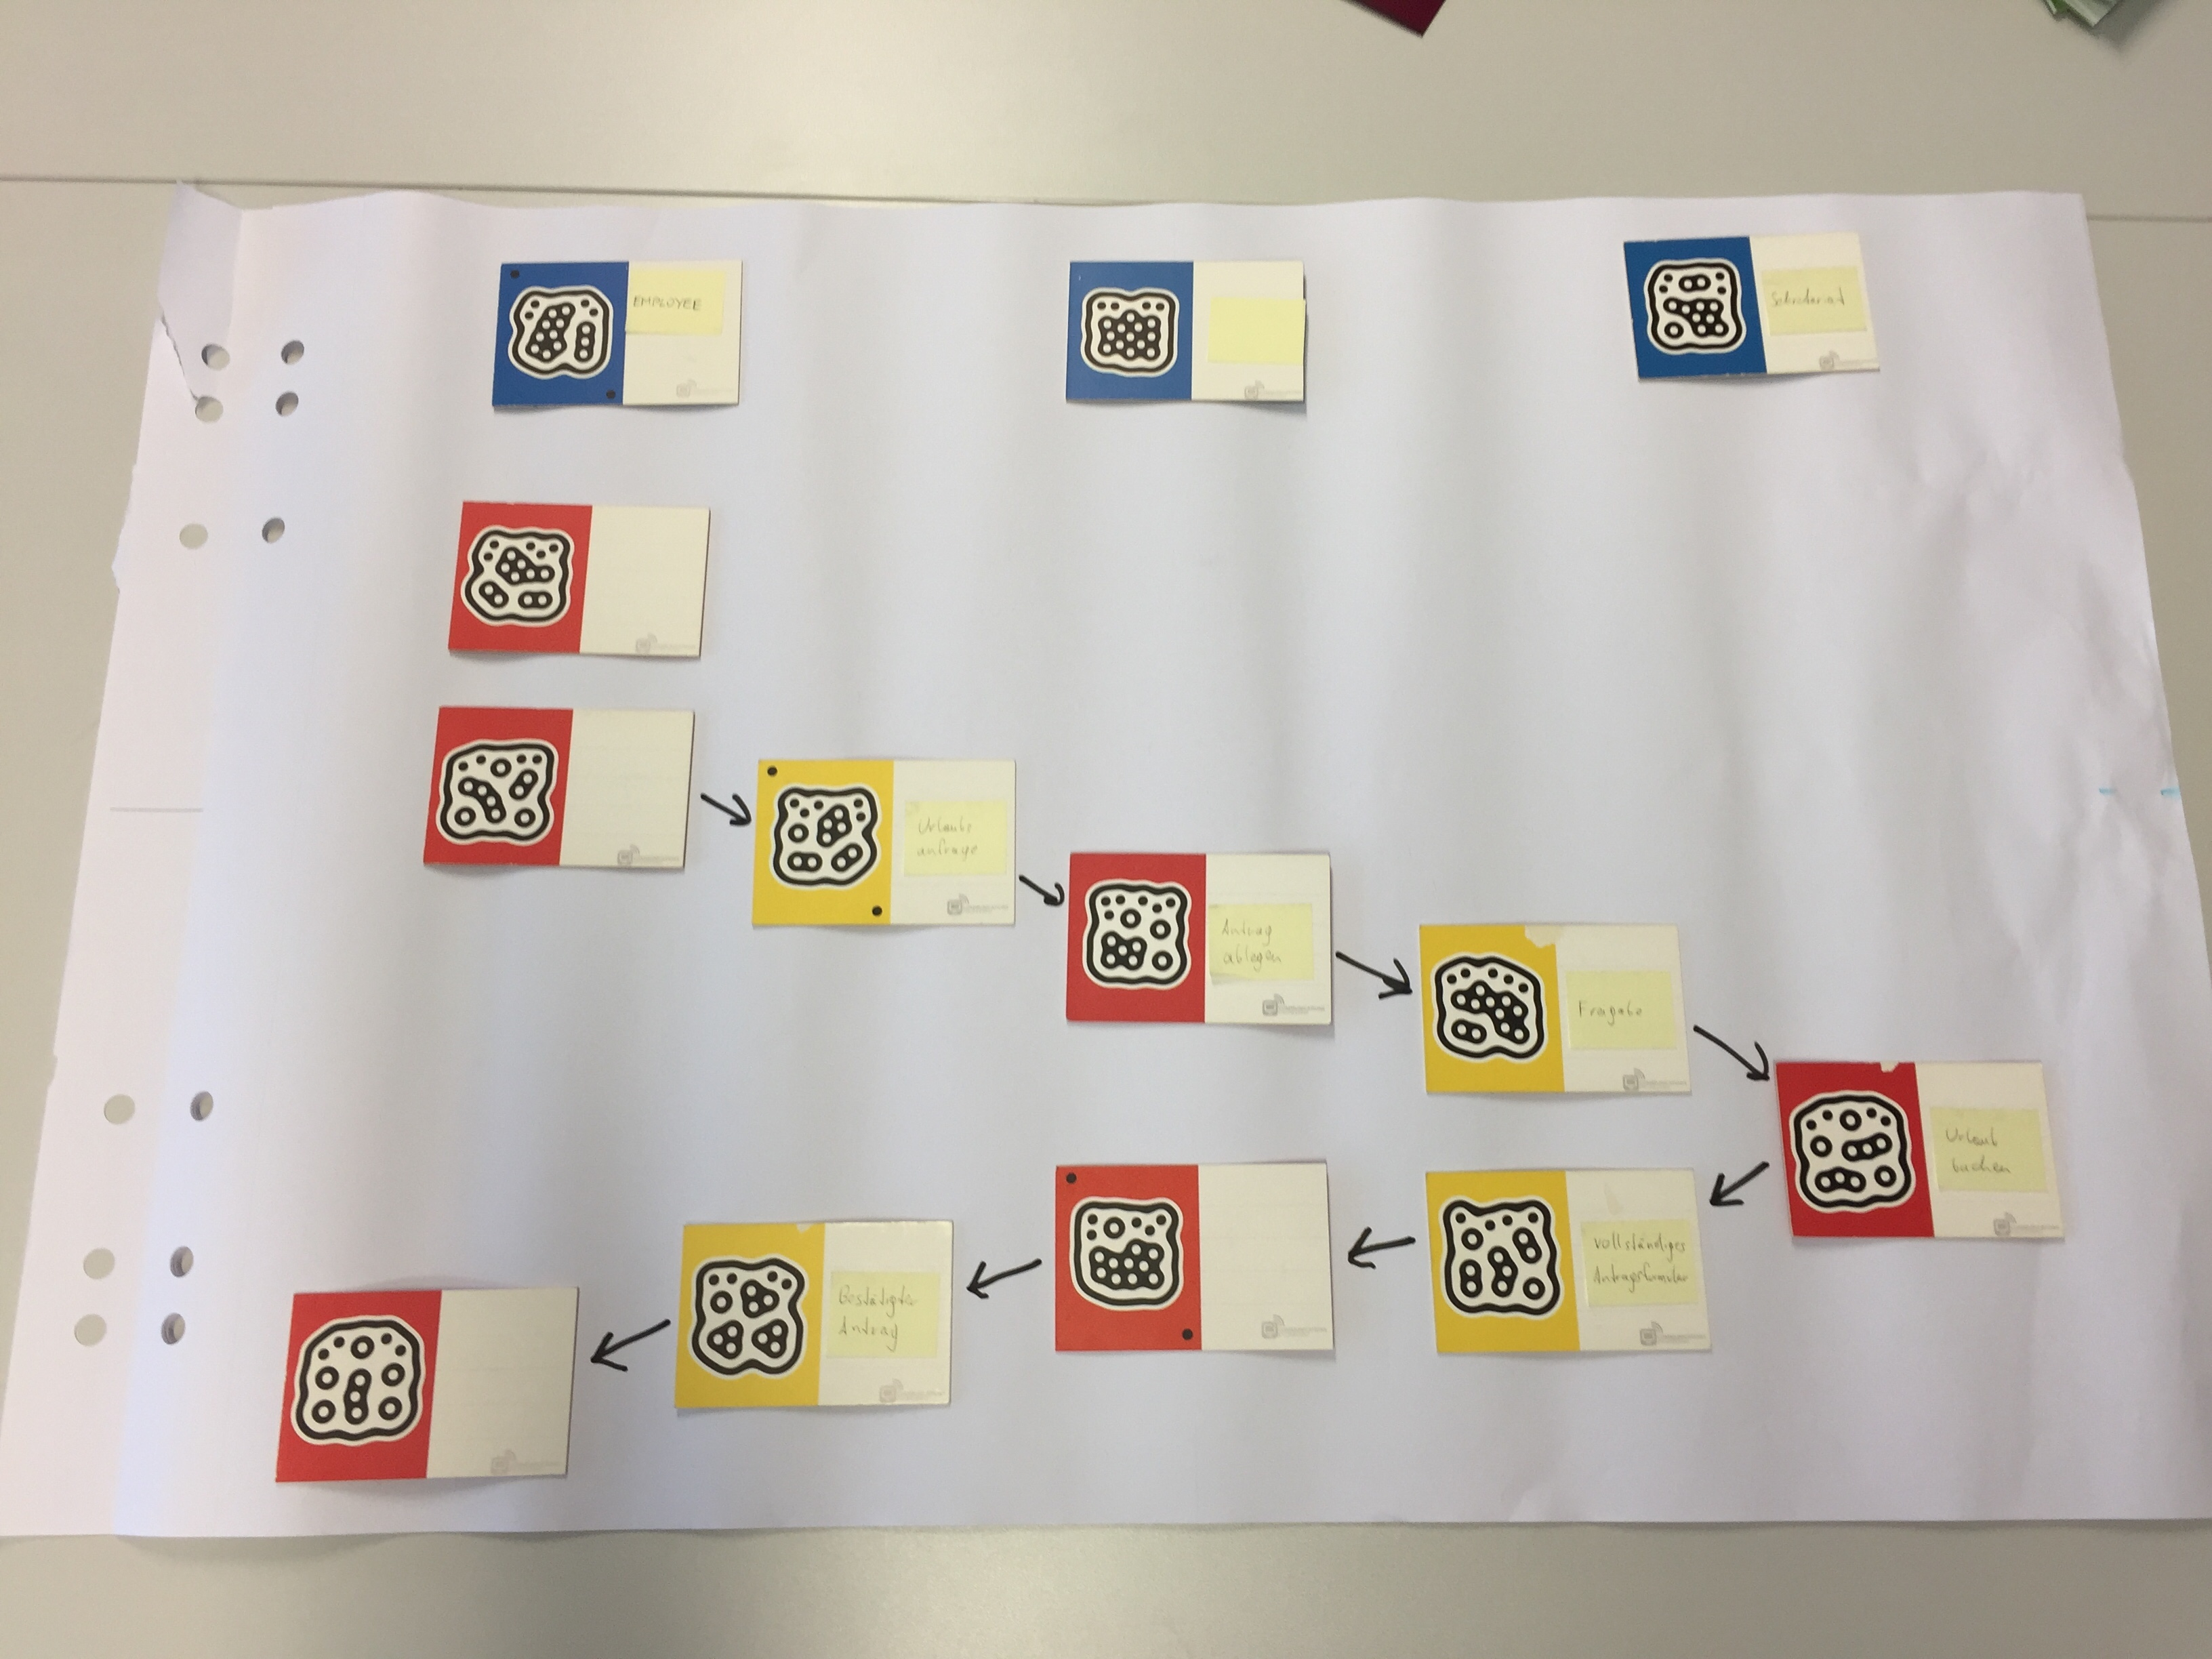
\includegraphics[width=\linewidth]{figures/01.jpg} & Ja & Dieses Beispiel entspricht den Kriterien der Legetechnik. \\
		\midrule
		2 & 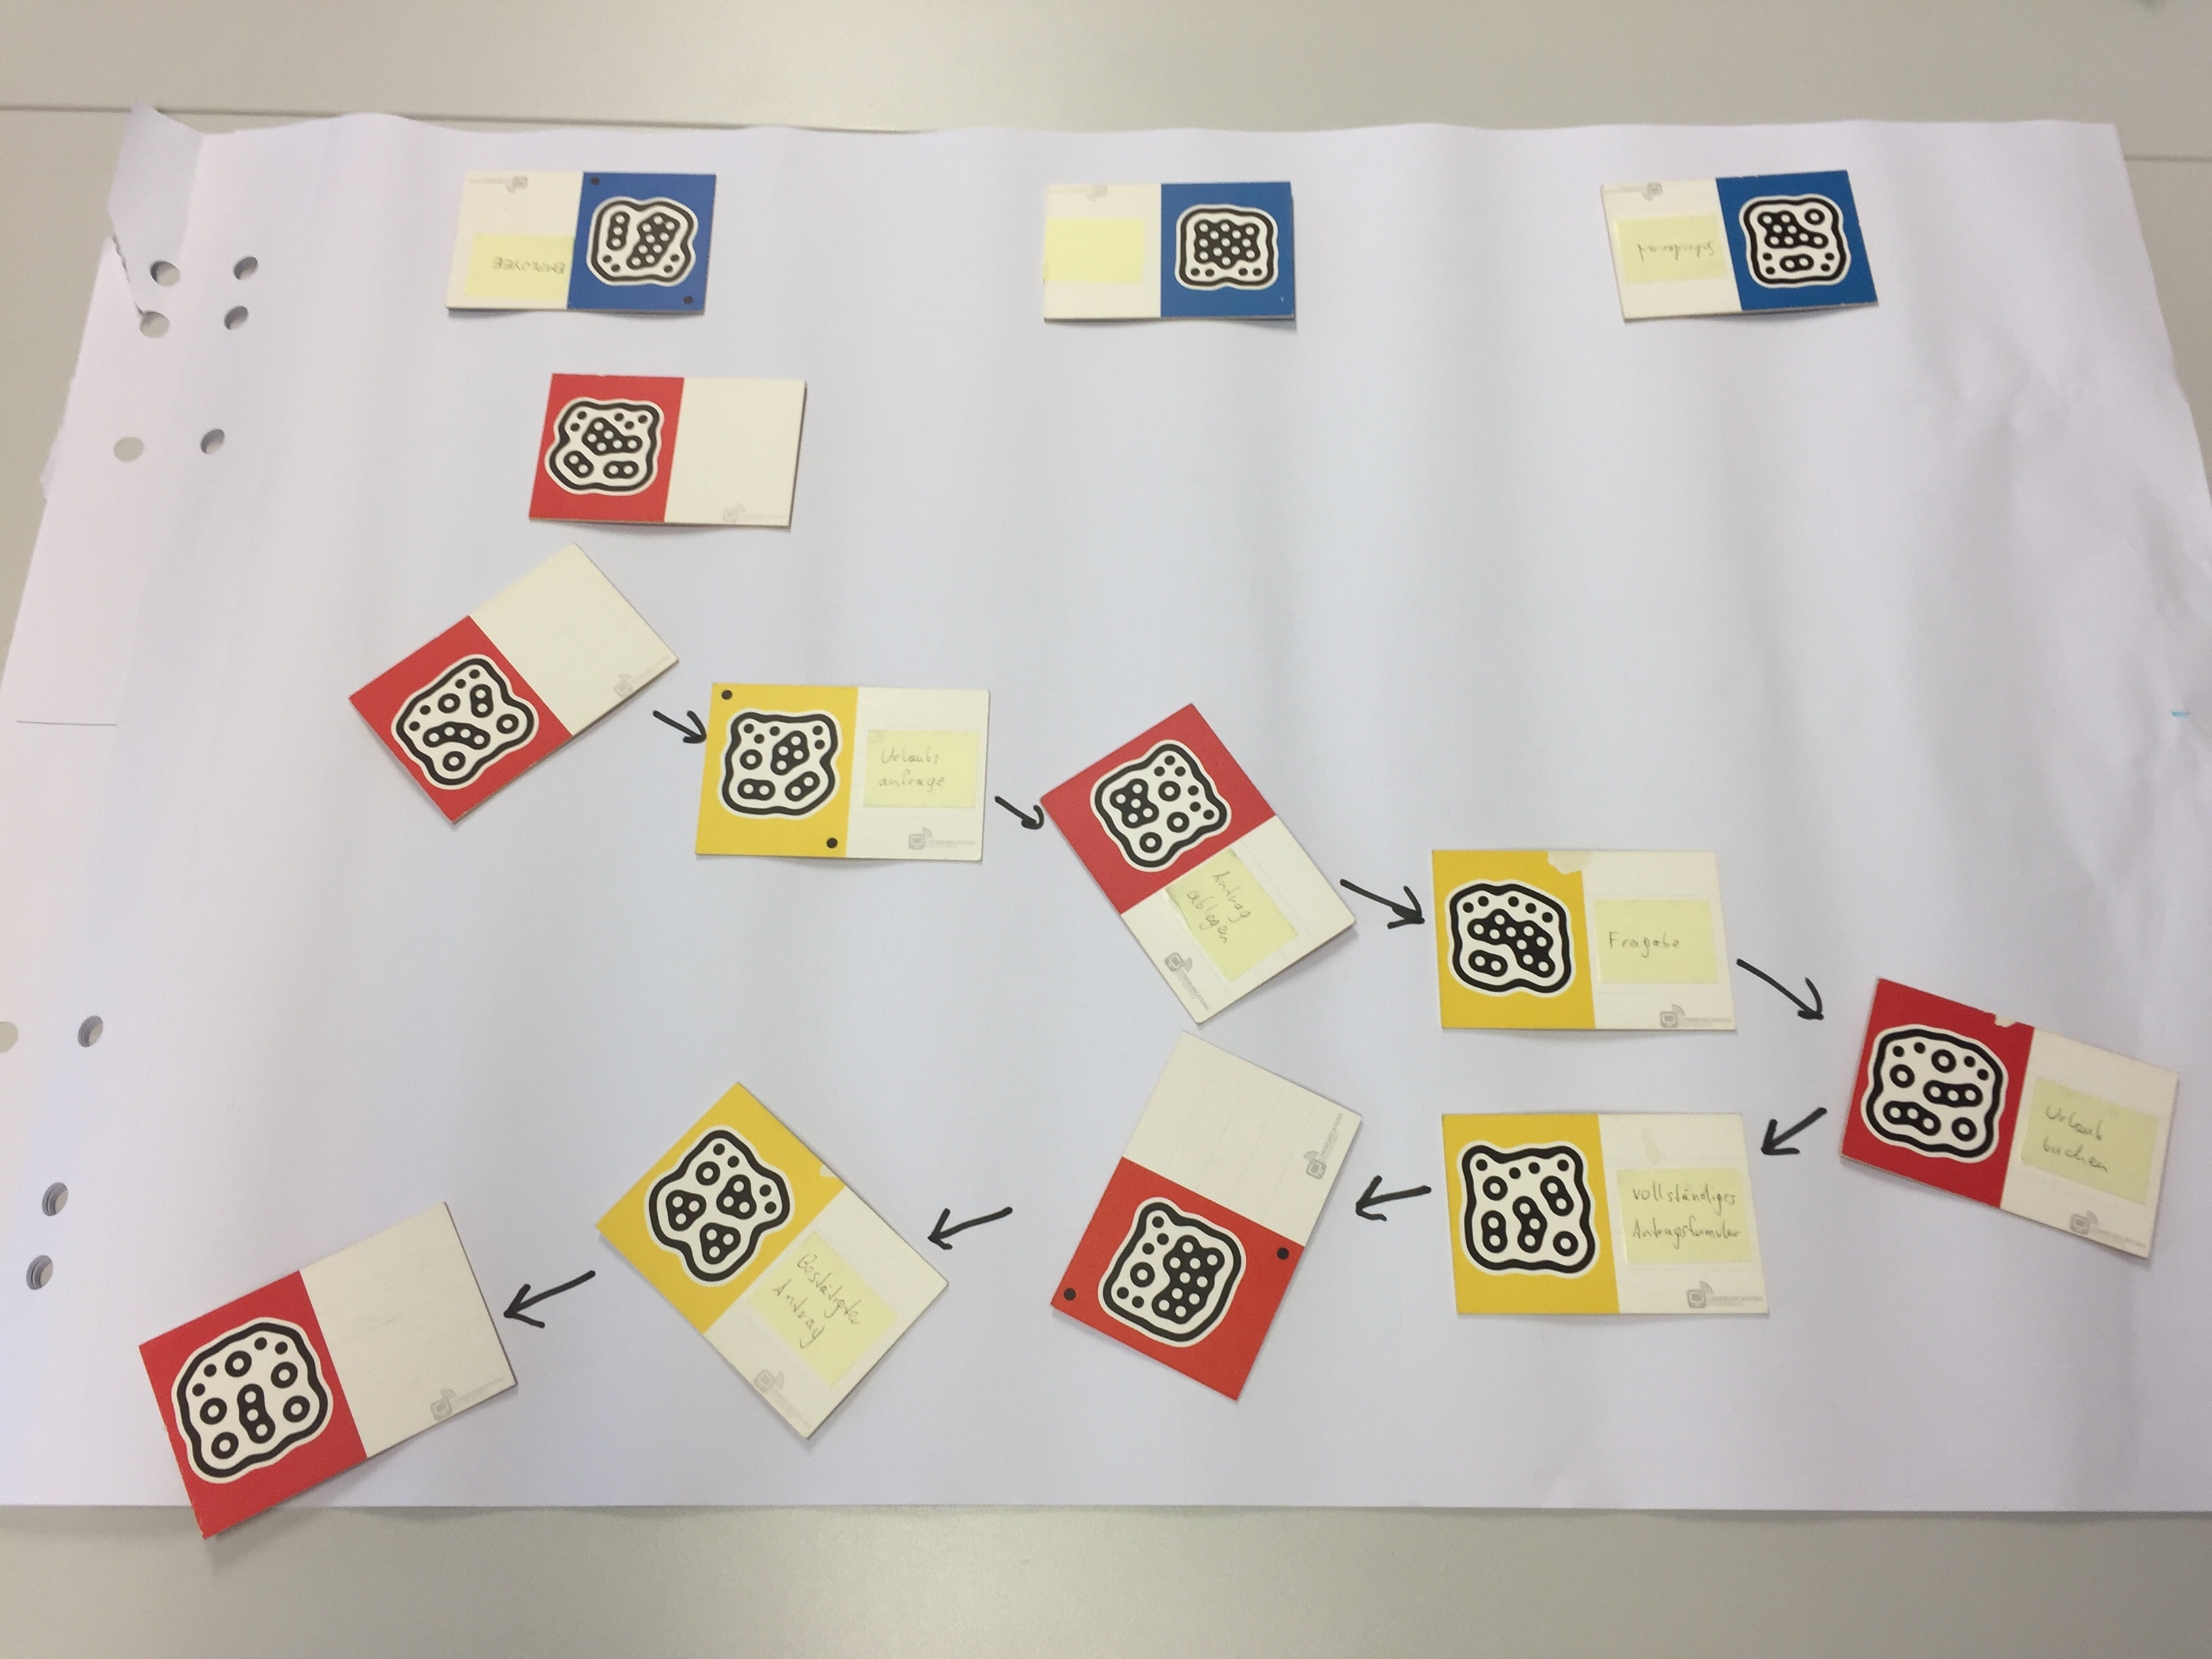
\includegraphics[width=\linewidth]{figures/02.jpg} & Ja & In diesem Beispiel ist ersichtlich, dass die Karten nicht exakt vertikal angeordnet sein müssen. \\
		\midrule
		3 & 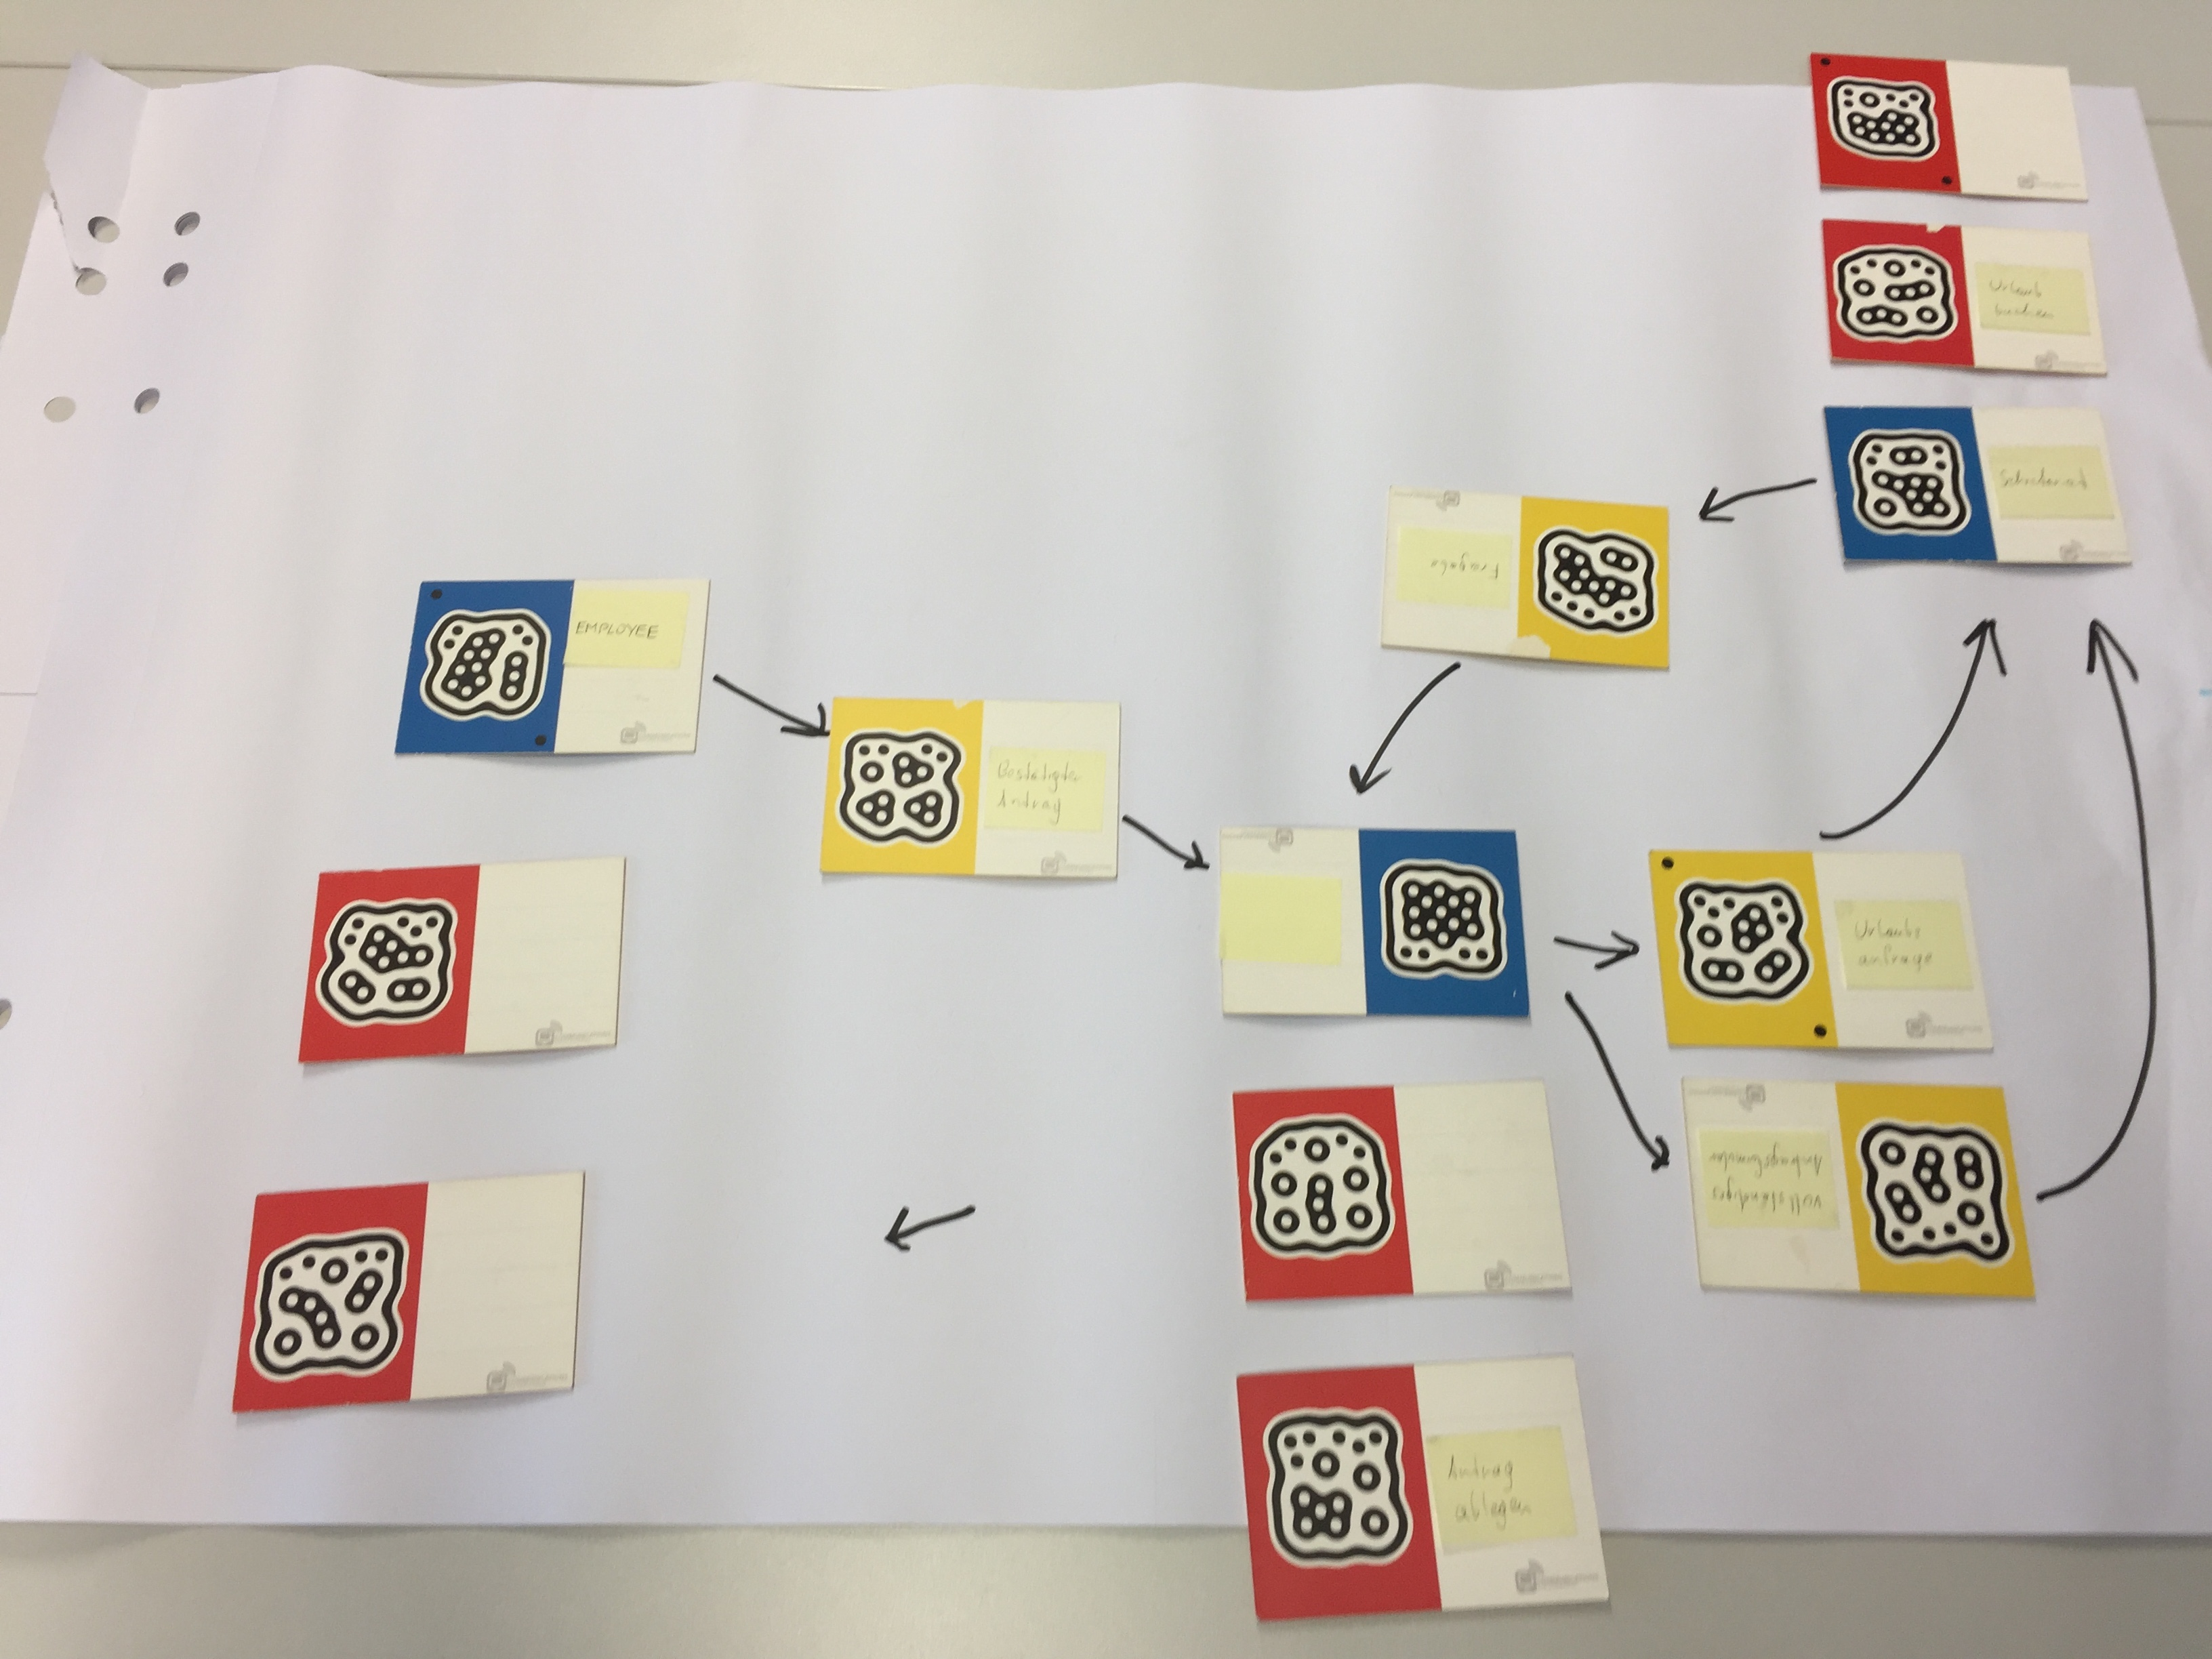
\includegraphics[width=\linewidth]{figures/03.jpg} & Ja & Die Lage der Subjekte ist für den Algorithmus nicht entscheidend. \\
		\midrule
		4 & 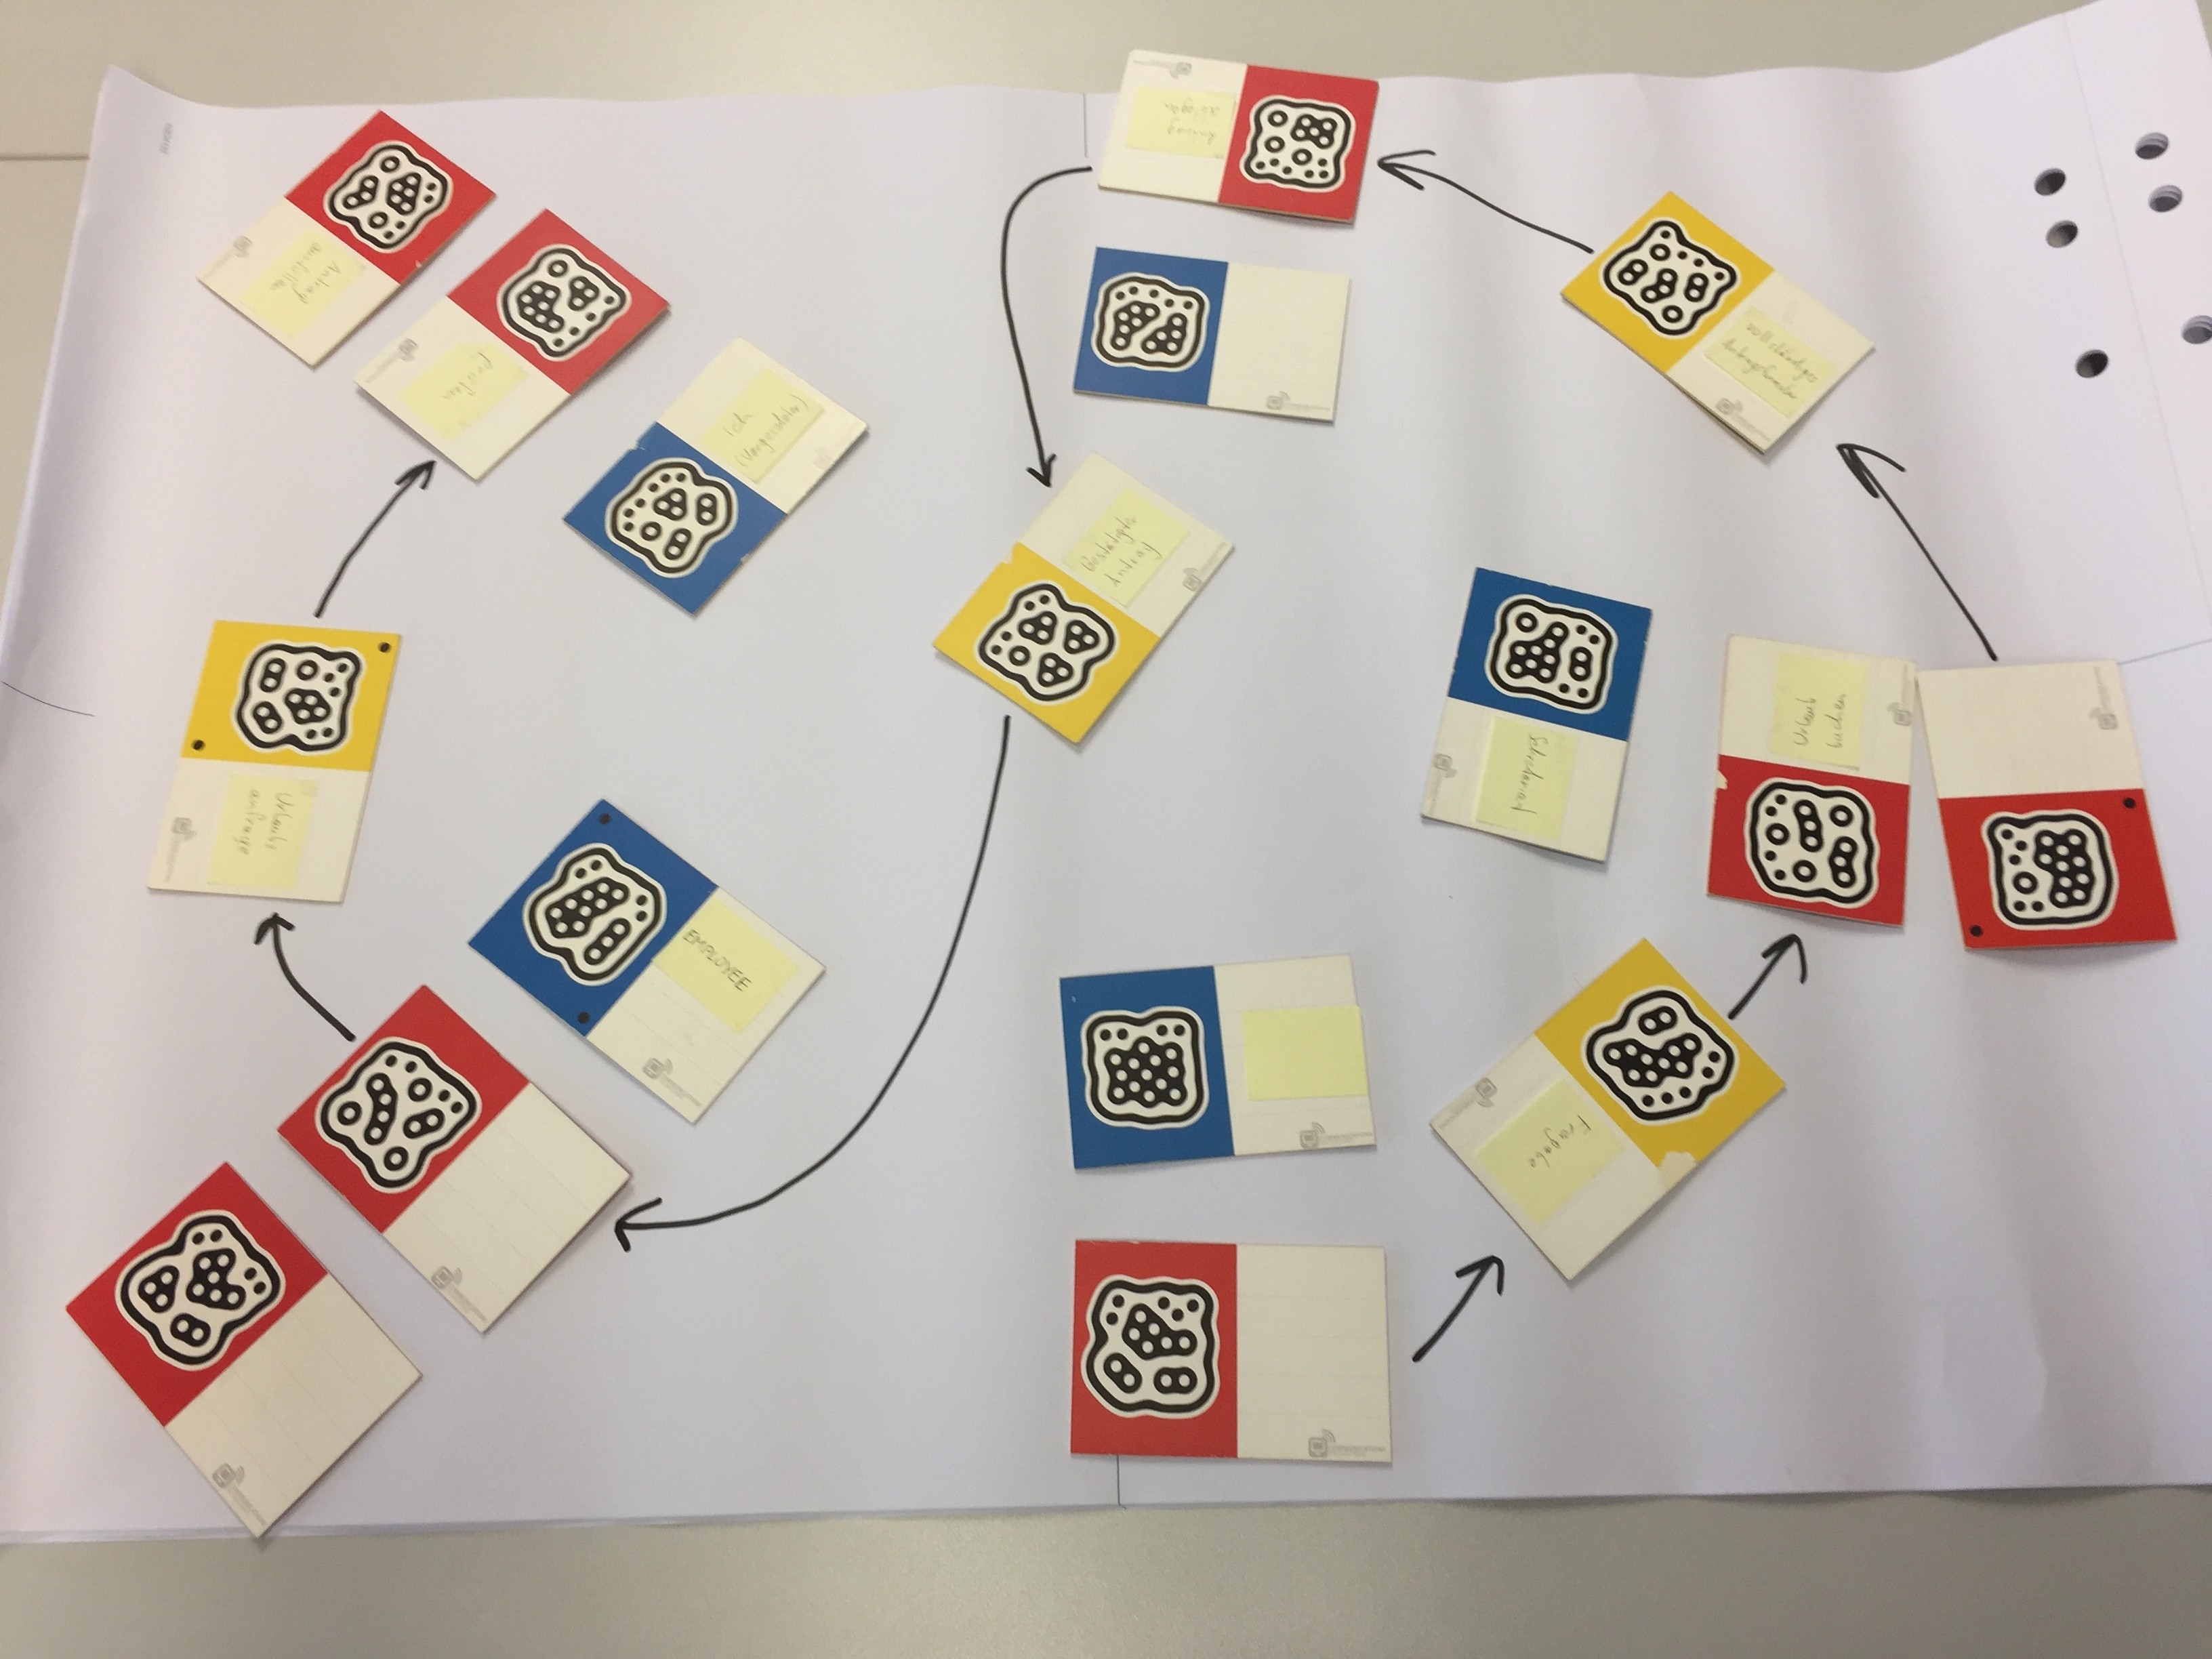
\includegraphics[width=\linewidth]{figures/04.jpg} & Ja & Dieses Beispiel ist dem Anschein nach als Sternmuster gelegt. Dennoch wird das Muster erkannt, da die Aufgaben jedes Subjekts in Linie gelegt sind. \\
		\midrule
		5 & 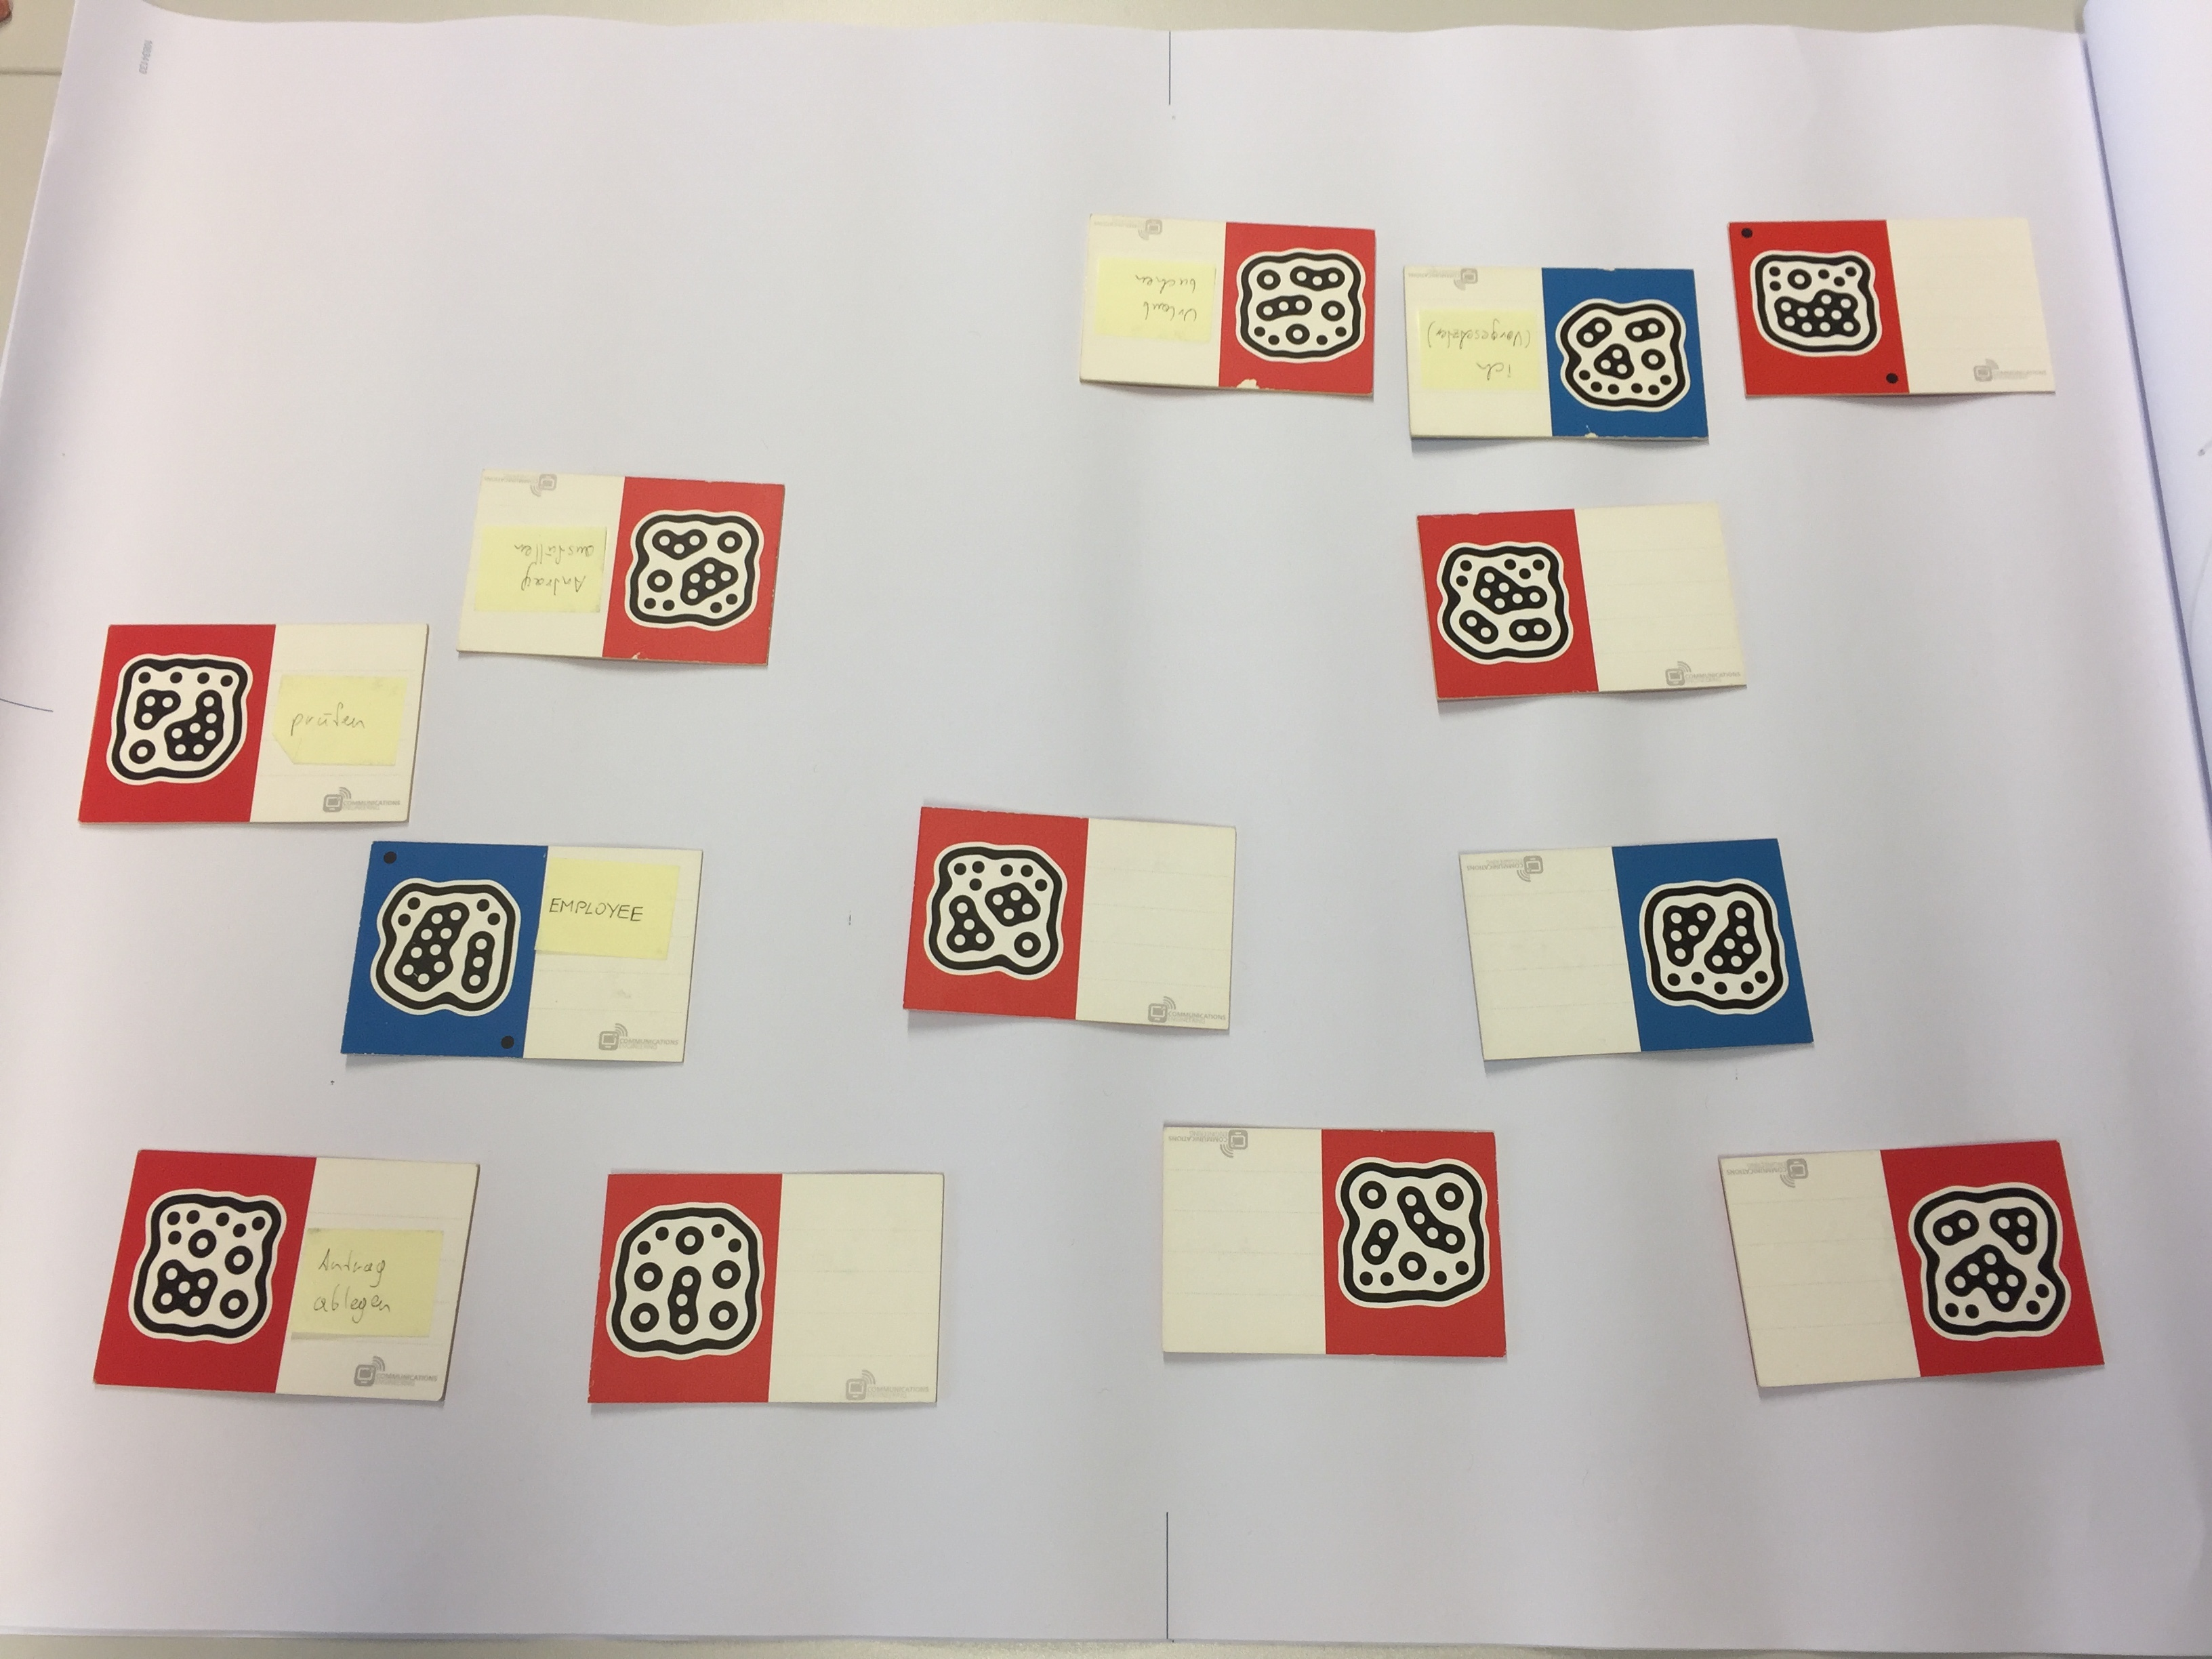
\includegraphics[width=\linewidth]{figures/05.jpg} & Ja & Der Testfall wird als Sternmuster erkannt. \\
		\midrule
		6 & 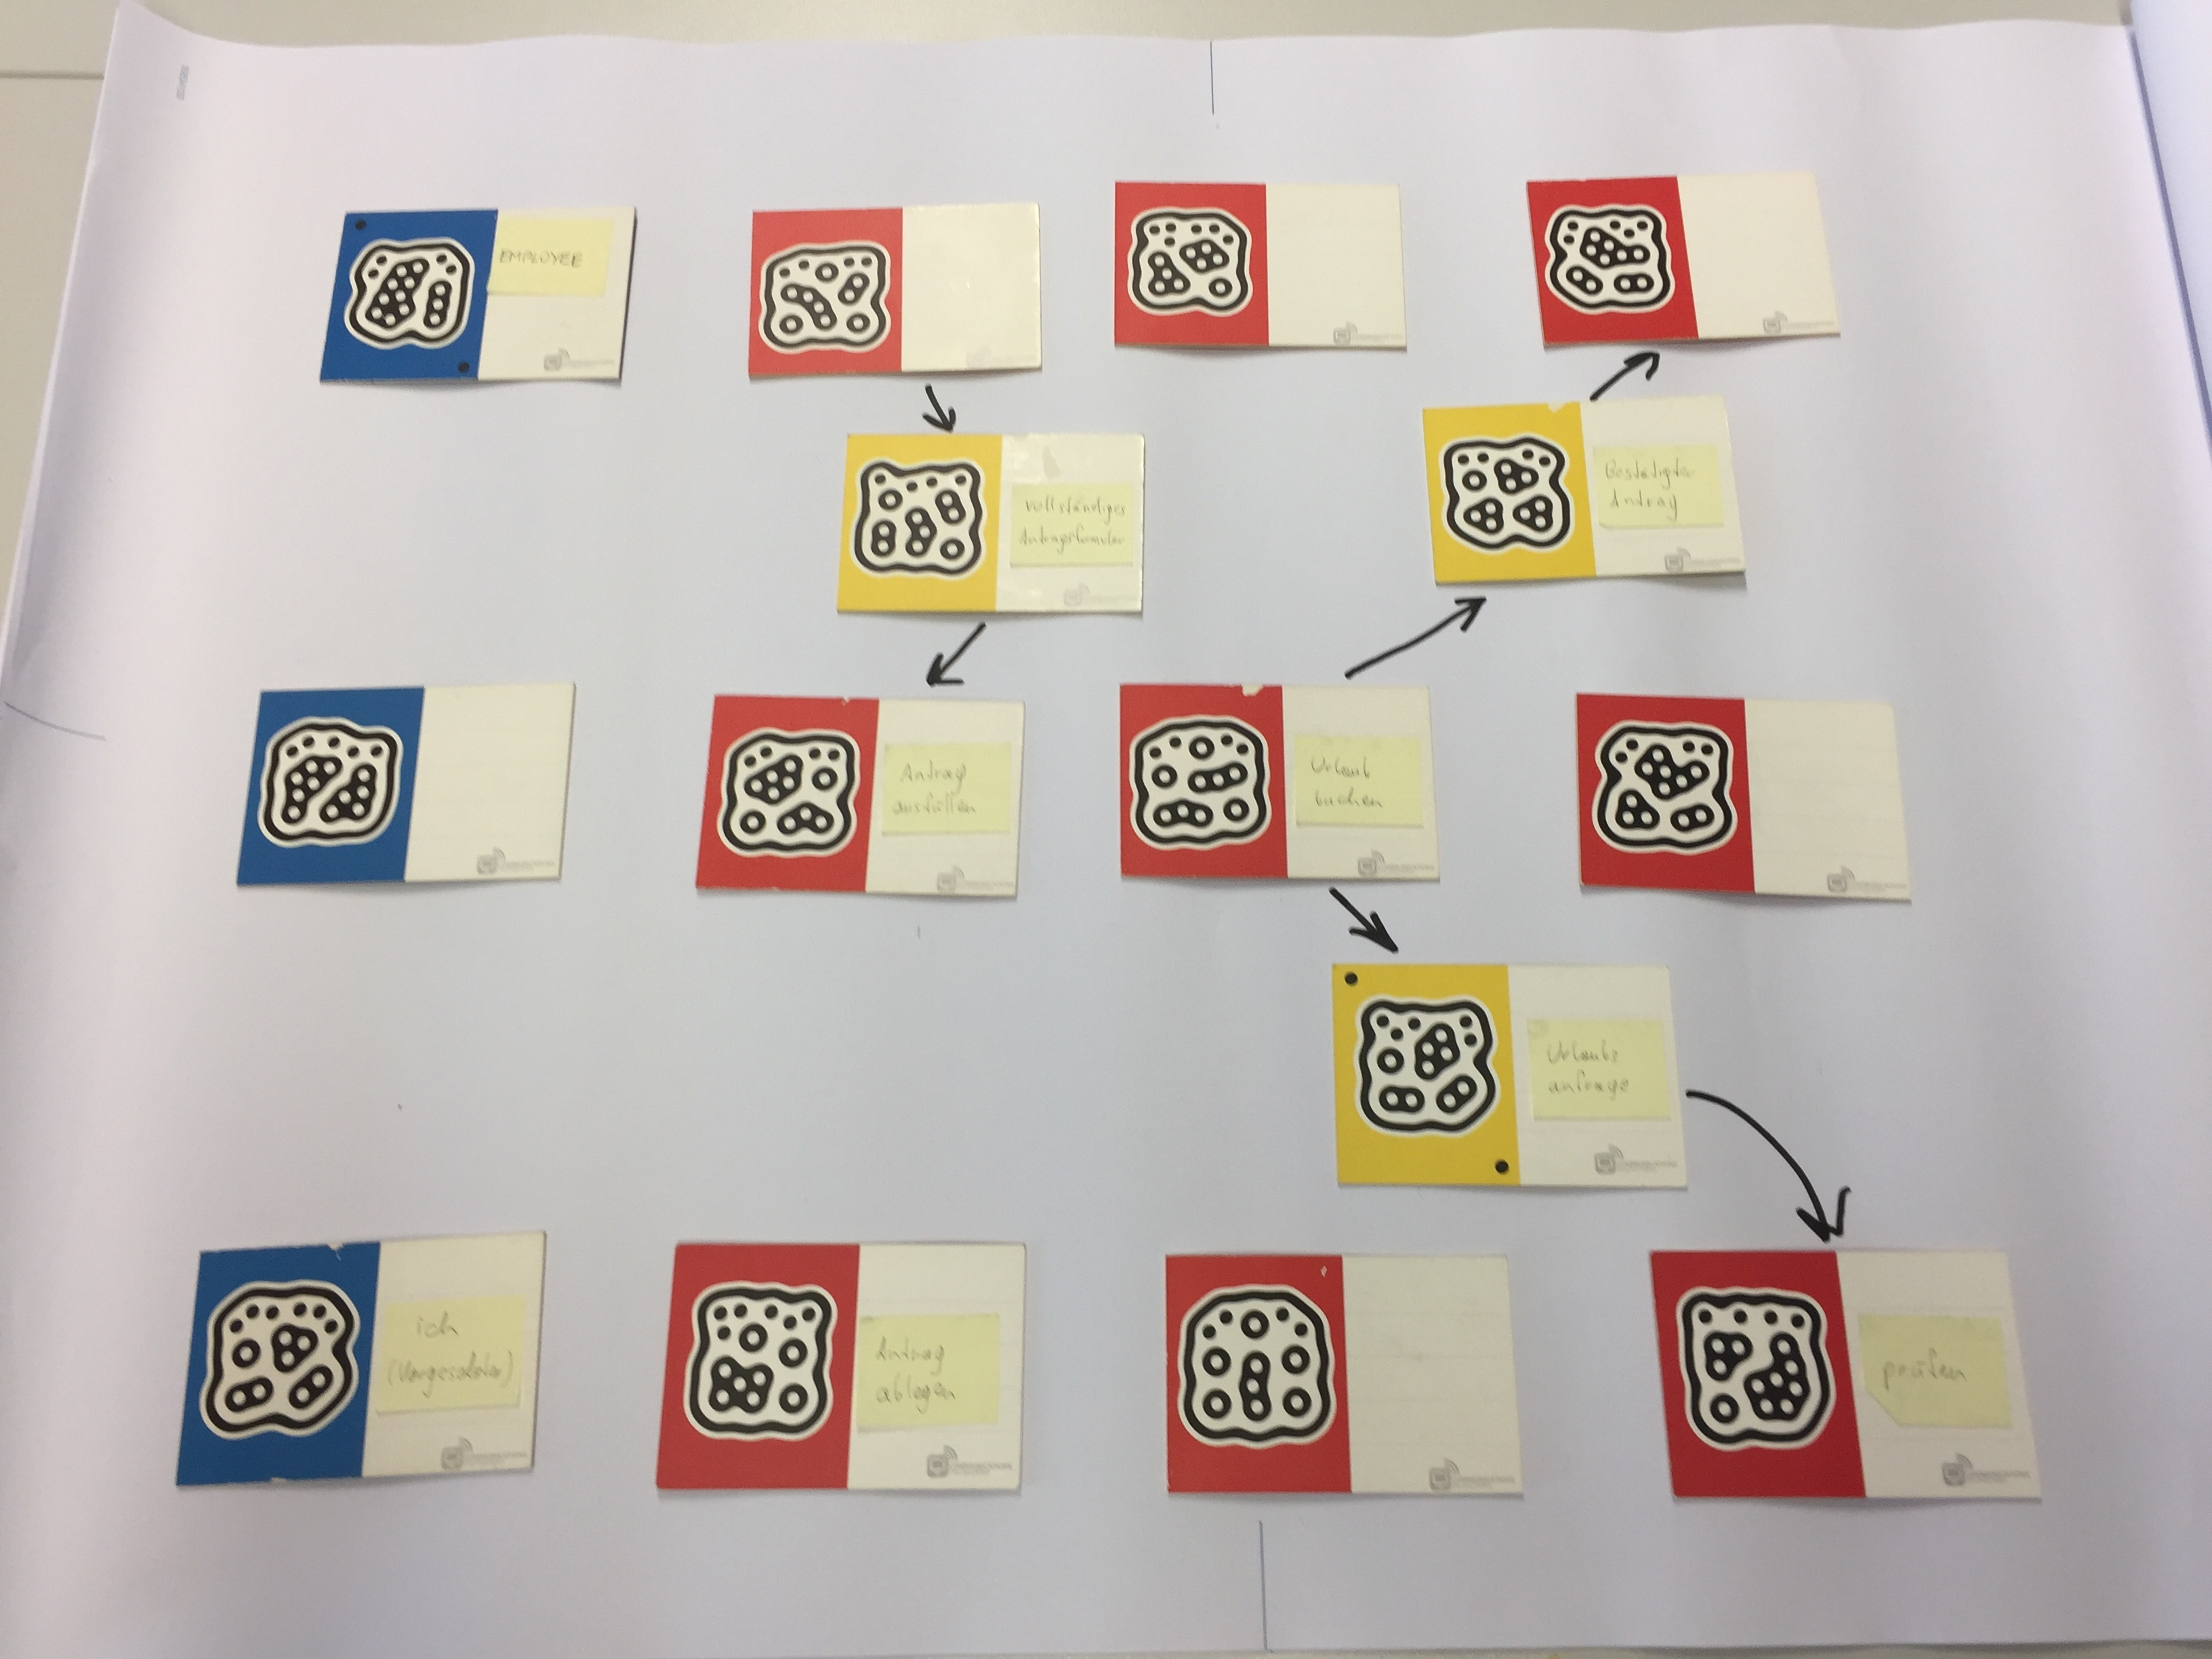
\includegraphics[width=\linewidth]{figures/06.jpg} & Ja & Der Testfall wird richtig erkannt. Die horizontale Ausrichtung der Aufgaben wirkt sich nicht auf das Ergebnis des Algorithmus aus. \\
		\midrule
		7 & 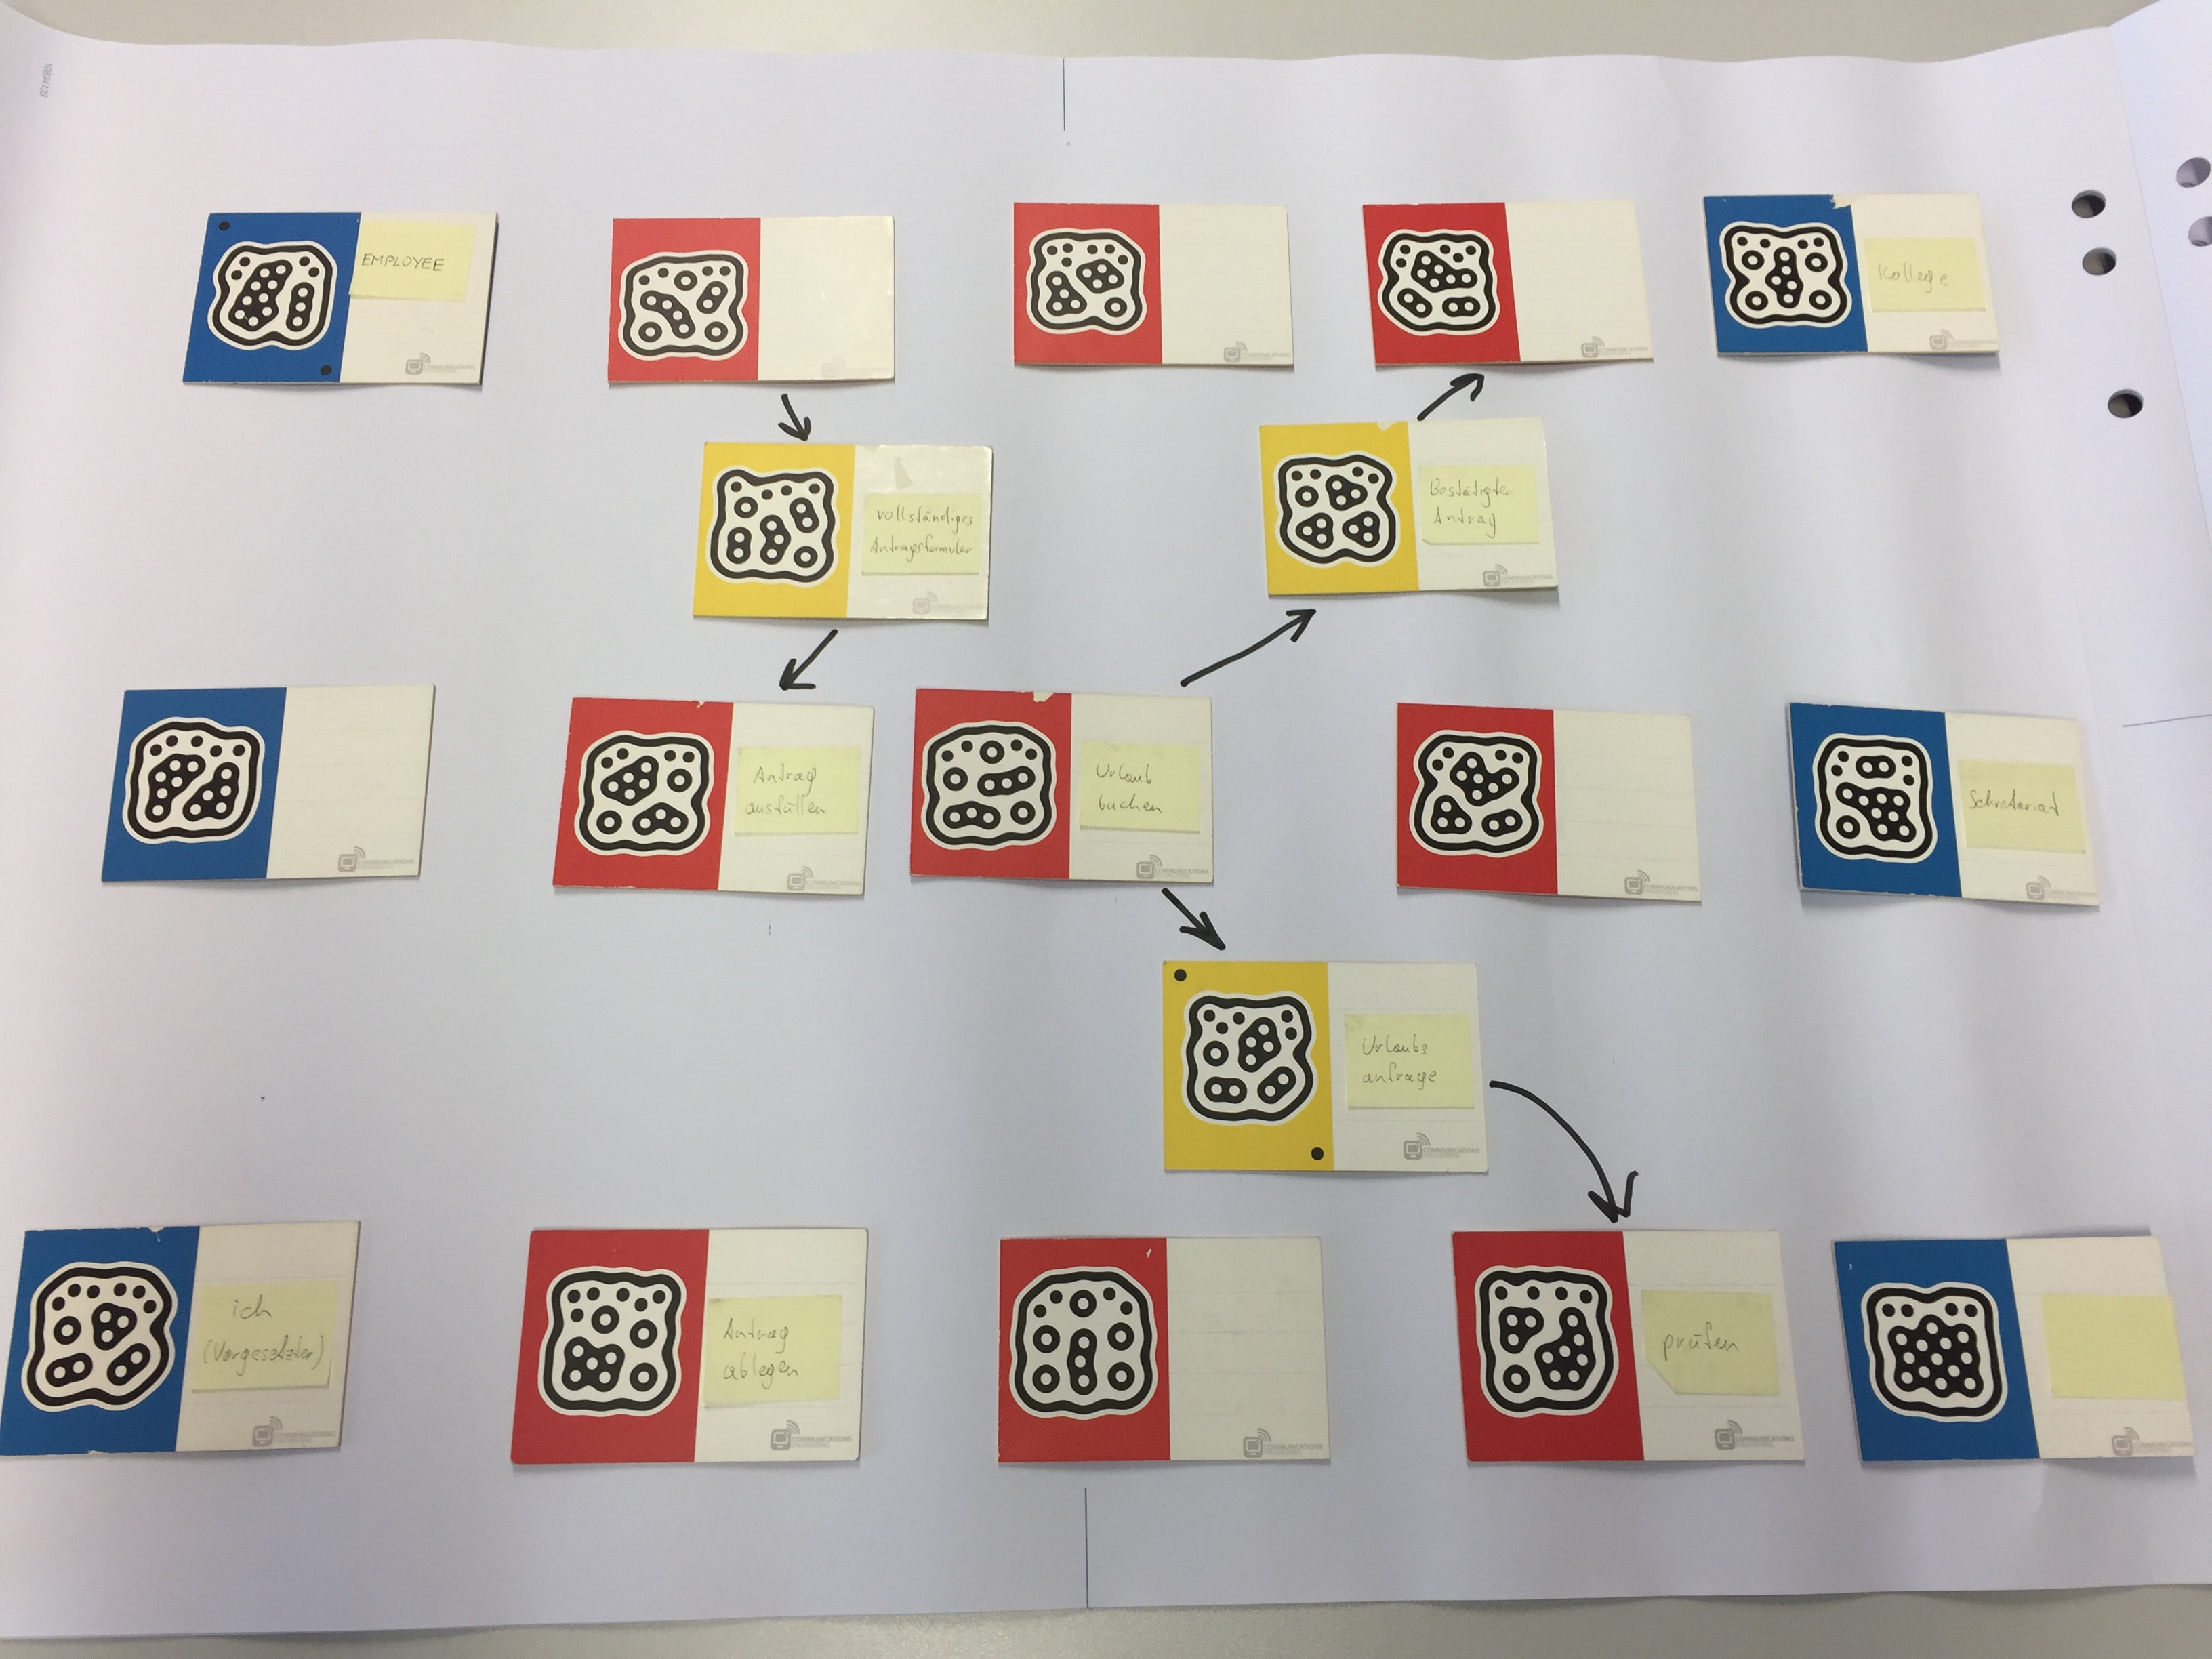
\includegraphics[width=\linewidth]{figures/07.jpg} & Ja & Der Testfall wird erkannt. Dabei werden die mittleren Aufgabenkarten korrekt über den minimalen Abstand zum Subjekt zugeordnet. \\
		\midrule
		8 & 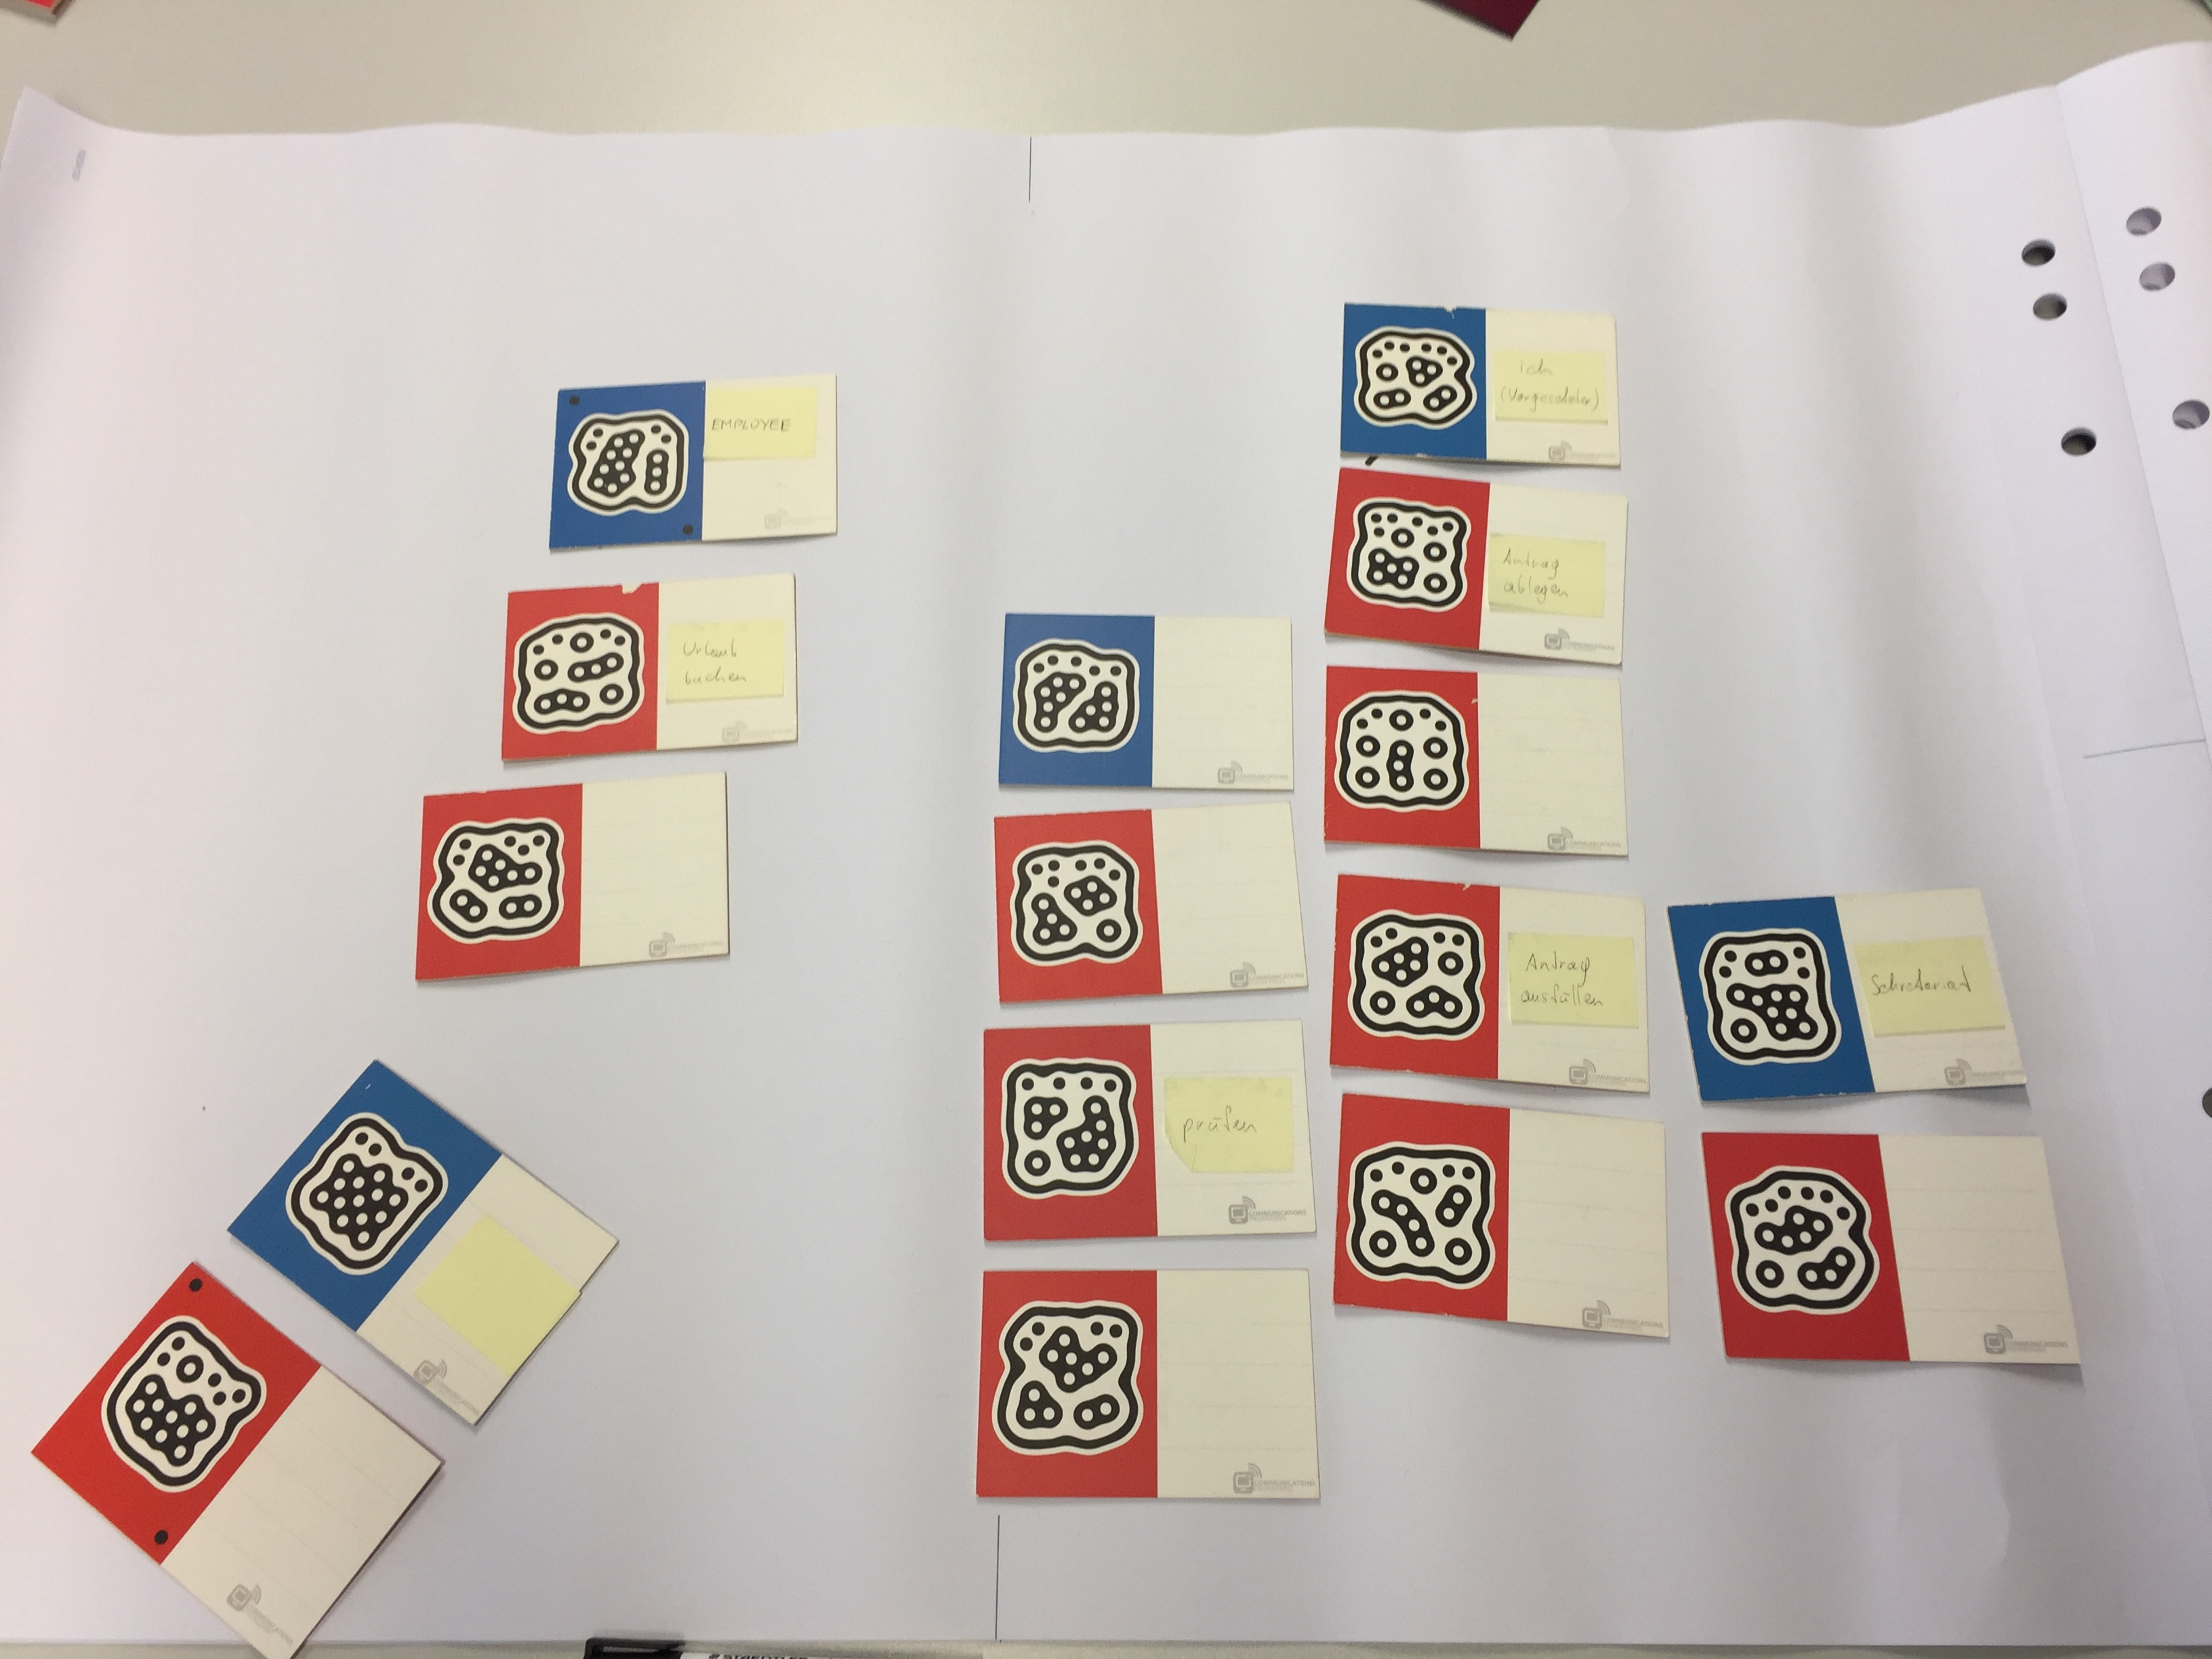
\includegraphics[width=\linewidth]{figures/08.jpg} & Ja & In diesem Beispiel wird die Aufgabe im linken unteren Eck korrekt zugeordnet, da der Vektor vom oberen linken Subjekt zur Aufgabe ein Subjekt schneidet.  \\
		\midrule
		9 & 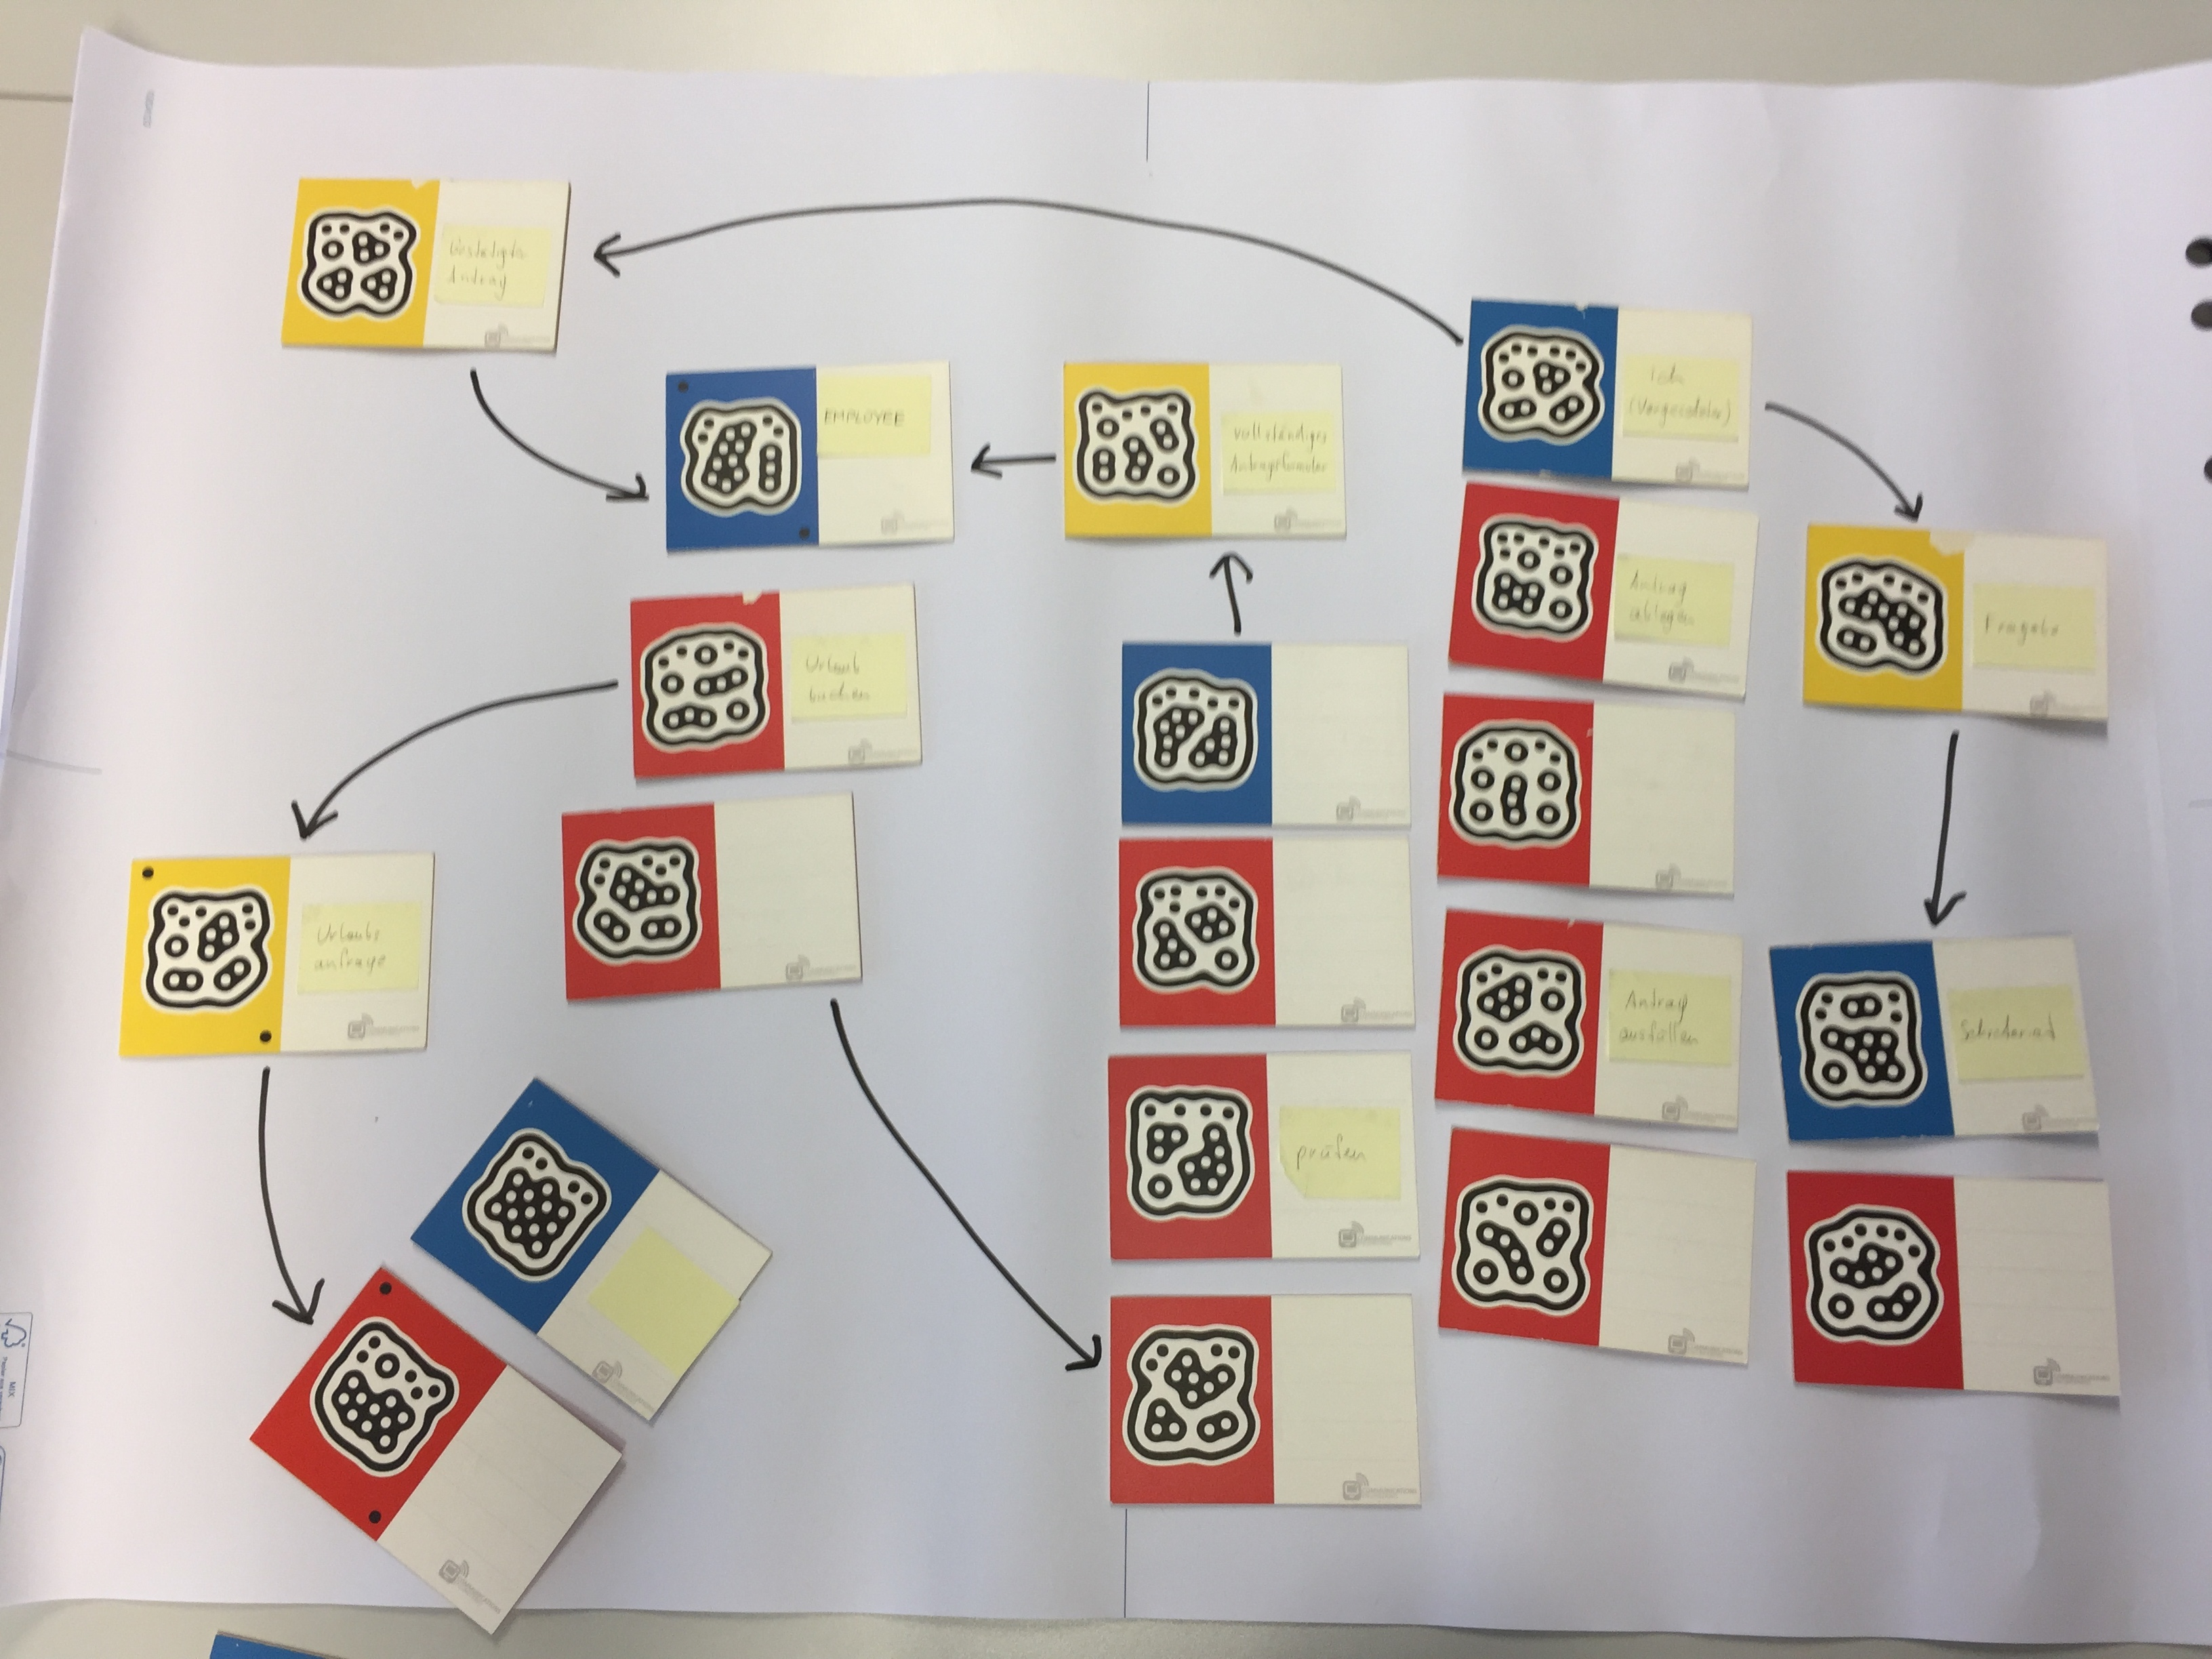
\includegraphics[width=\linewidth]{figures/09.jpg} & Ja & Entspricht in Bezug auf den Algorithmus dem Testfall 8. \\
		\midrule
		10 & 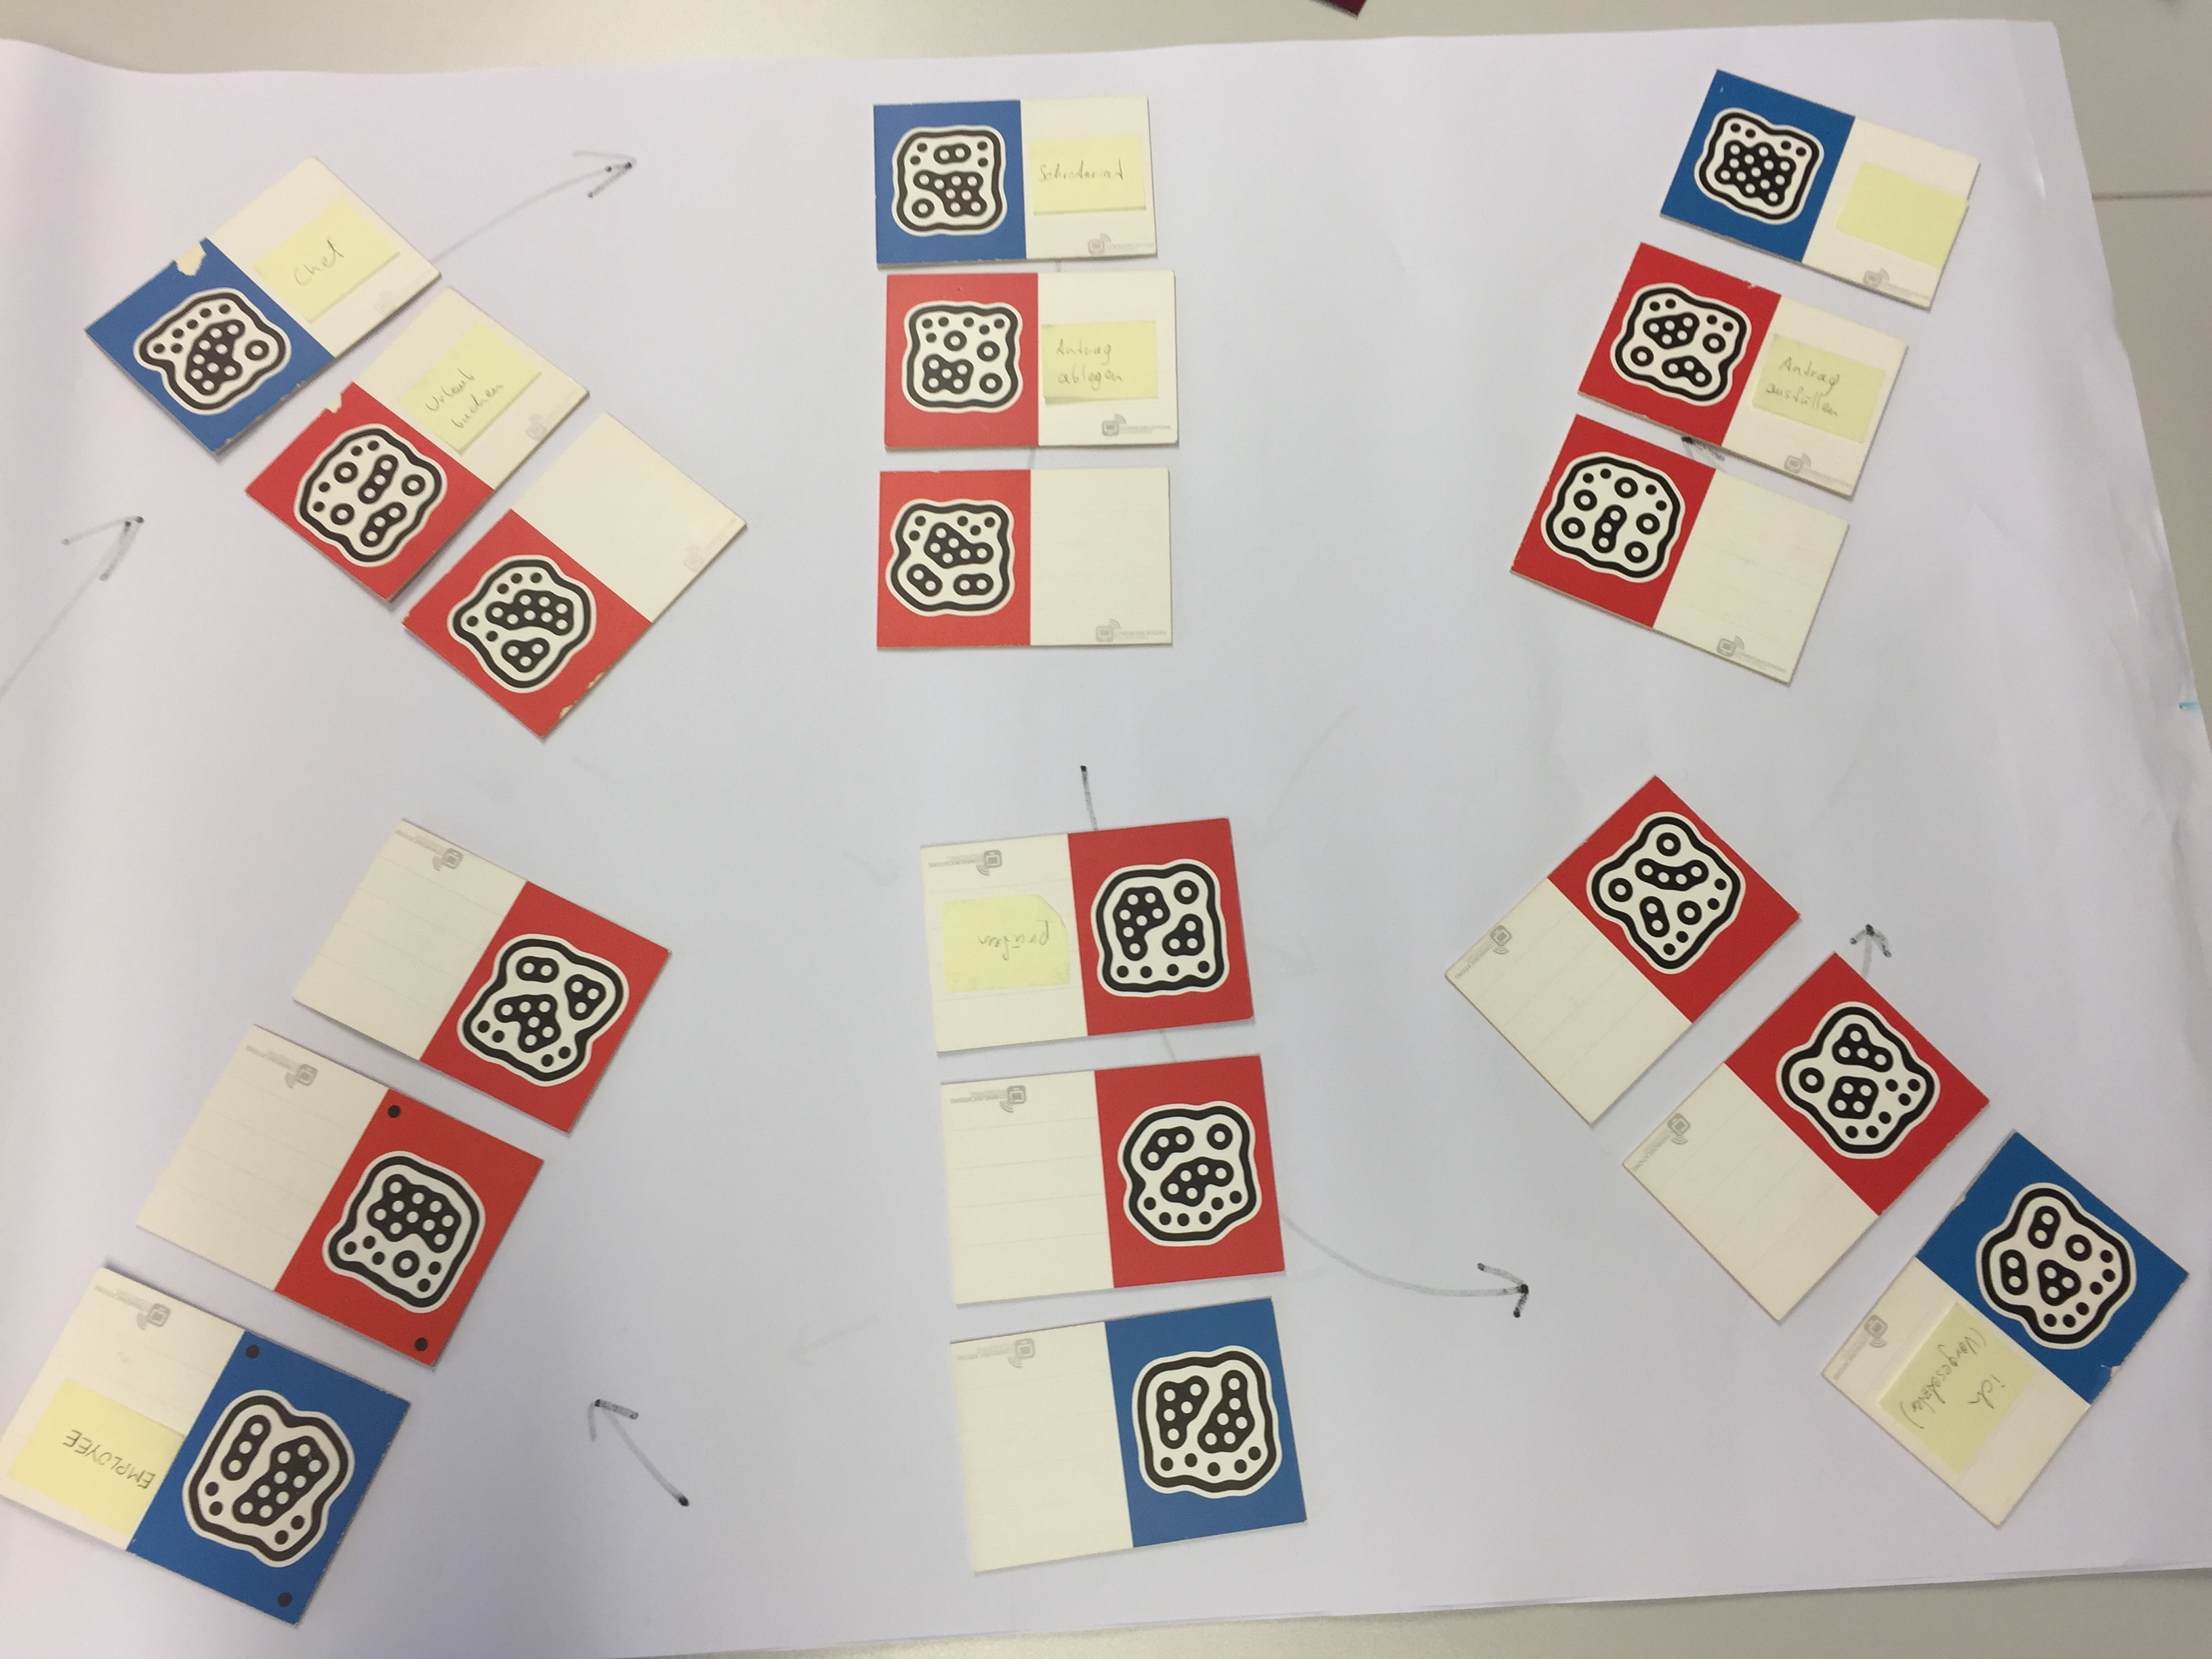
\includegraphics[width=\linewidth]{figures/10.jpg} & Ja & Dieses Beispiel ist scheinbar auch ein Sternmuster, wird aber korrekt als Linienmuster erkannt. In diesem Fall ist wird besonders die Funktionalität der Verifizierung geprüft. \\
		\midrule
		11 & 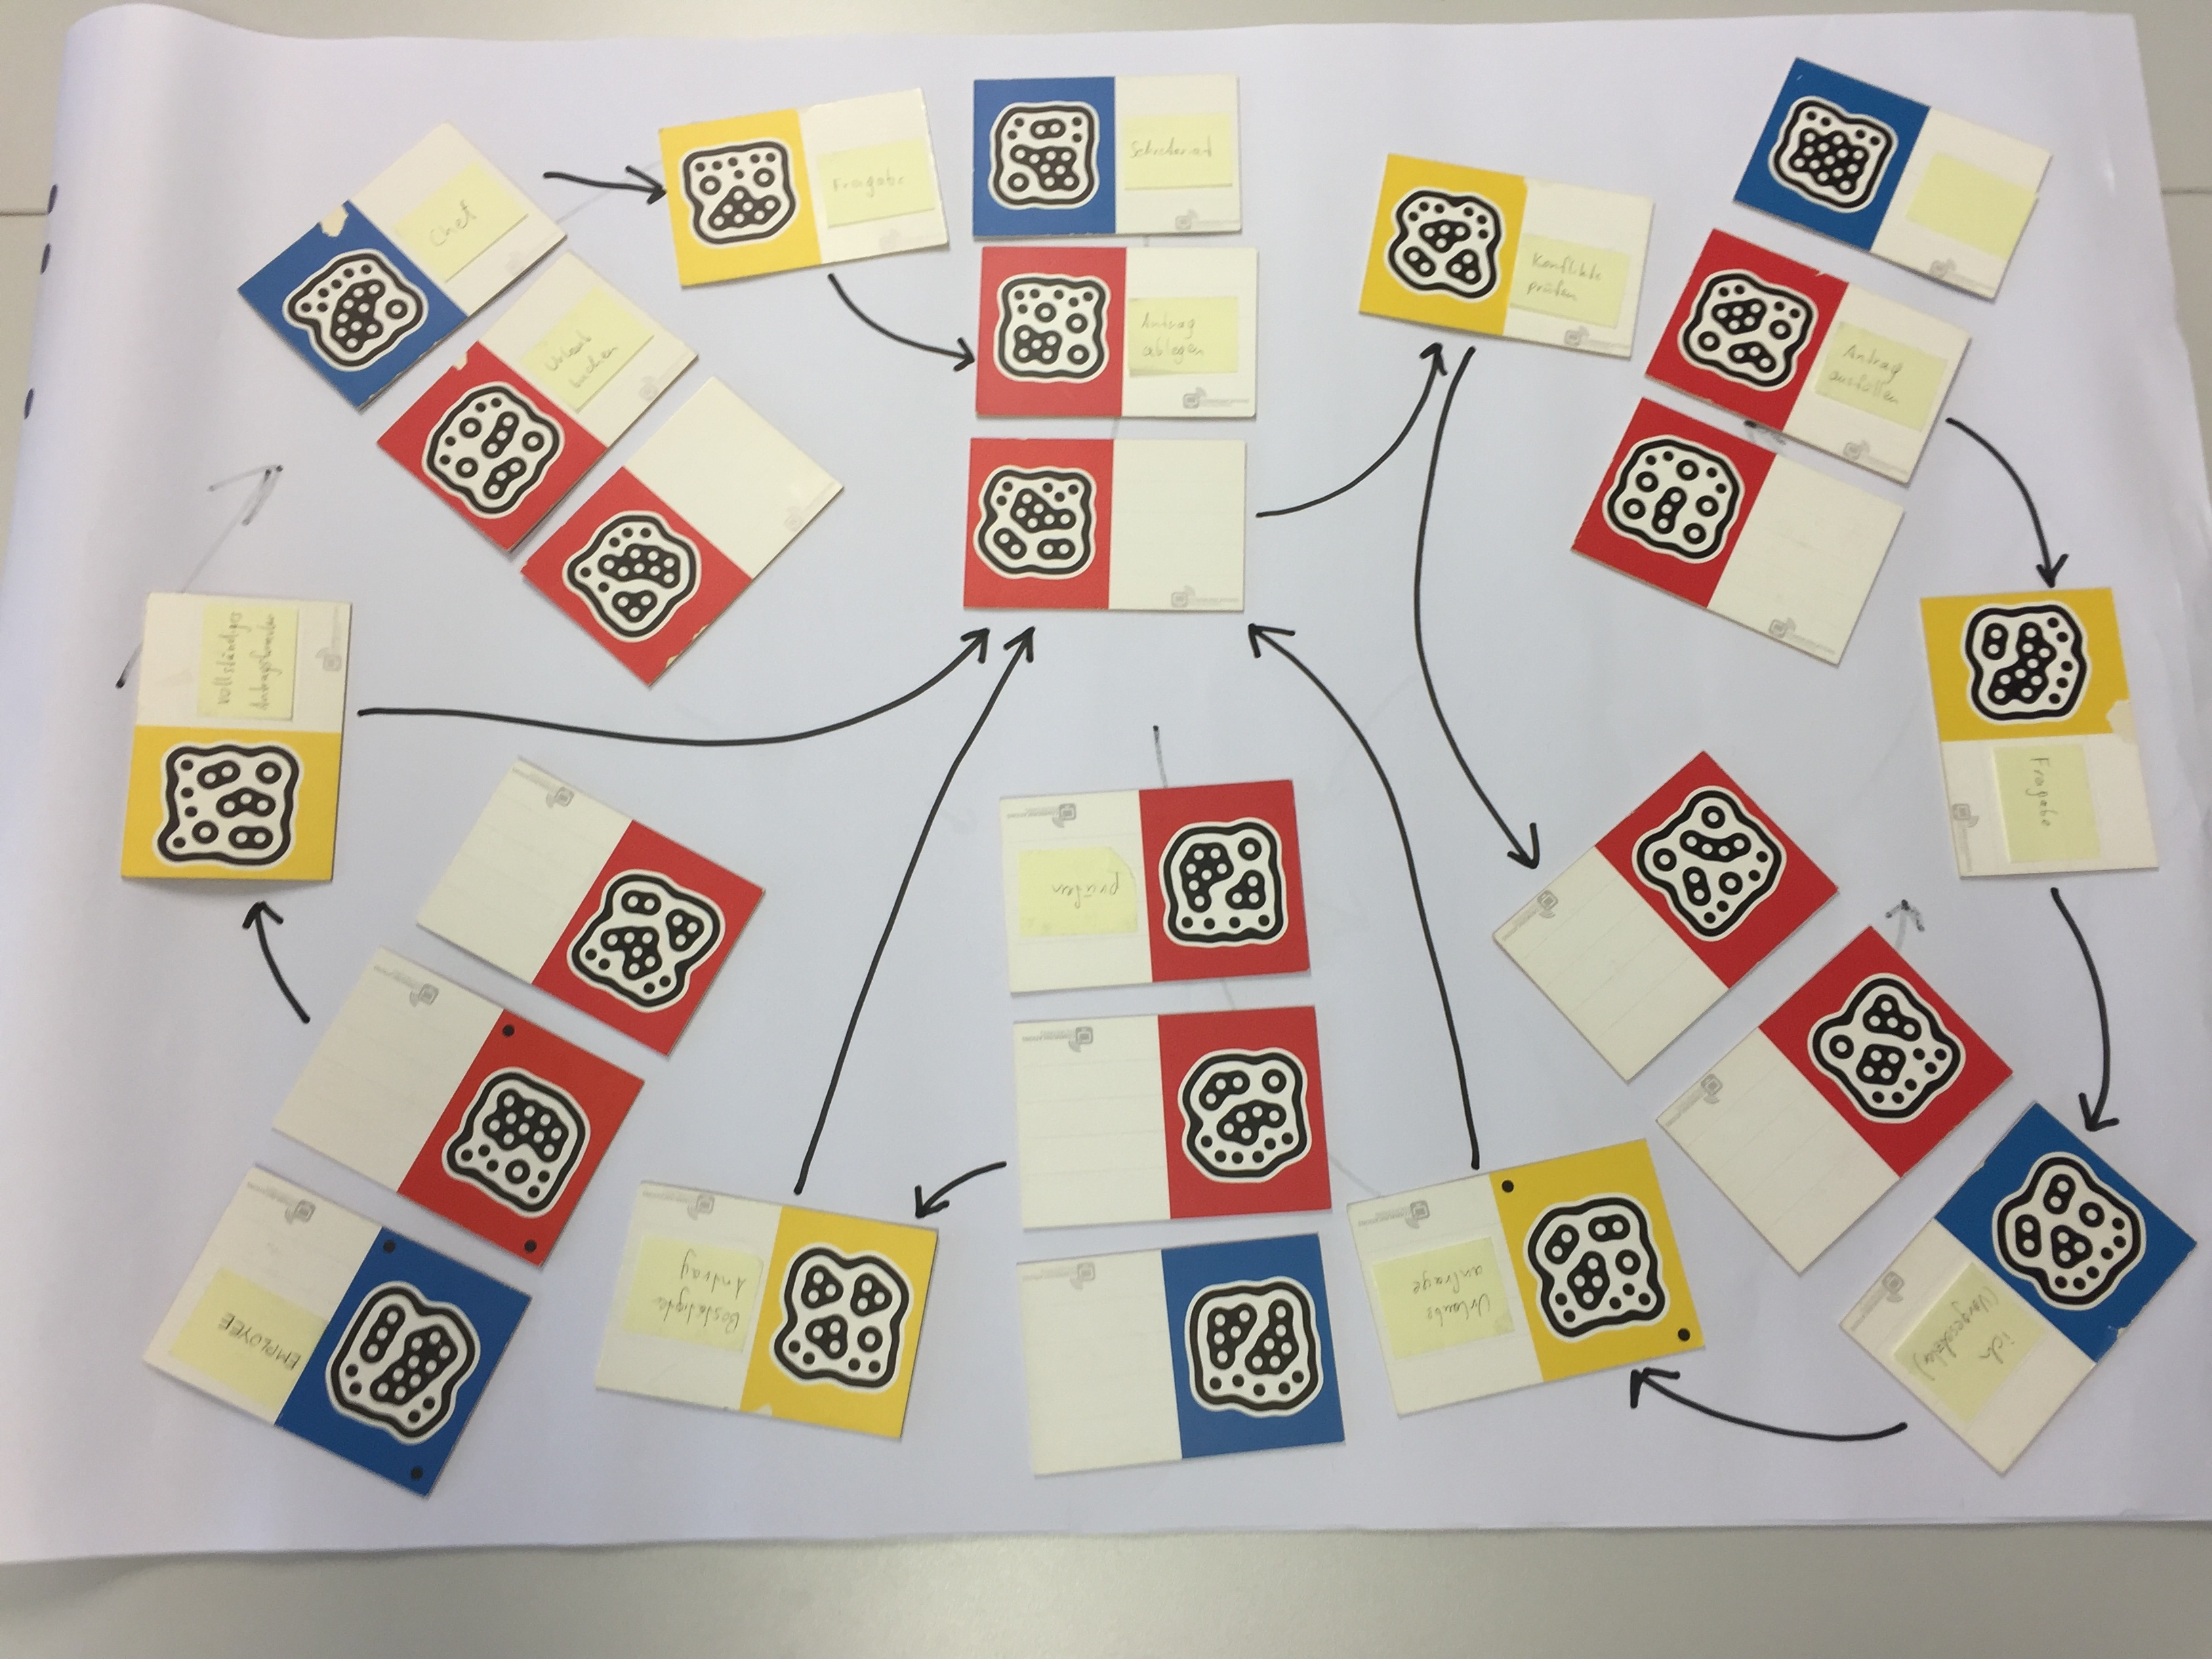
\includegraphics[width=\linewidth]{figures/11.jpg} & Ja & Entspricht in Bezug auf den Algorithmus dem Testfall 10.  \\
		\midrule
		12 & 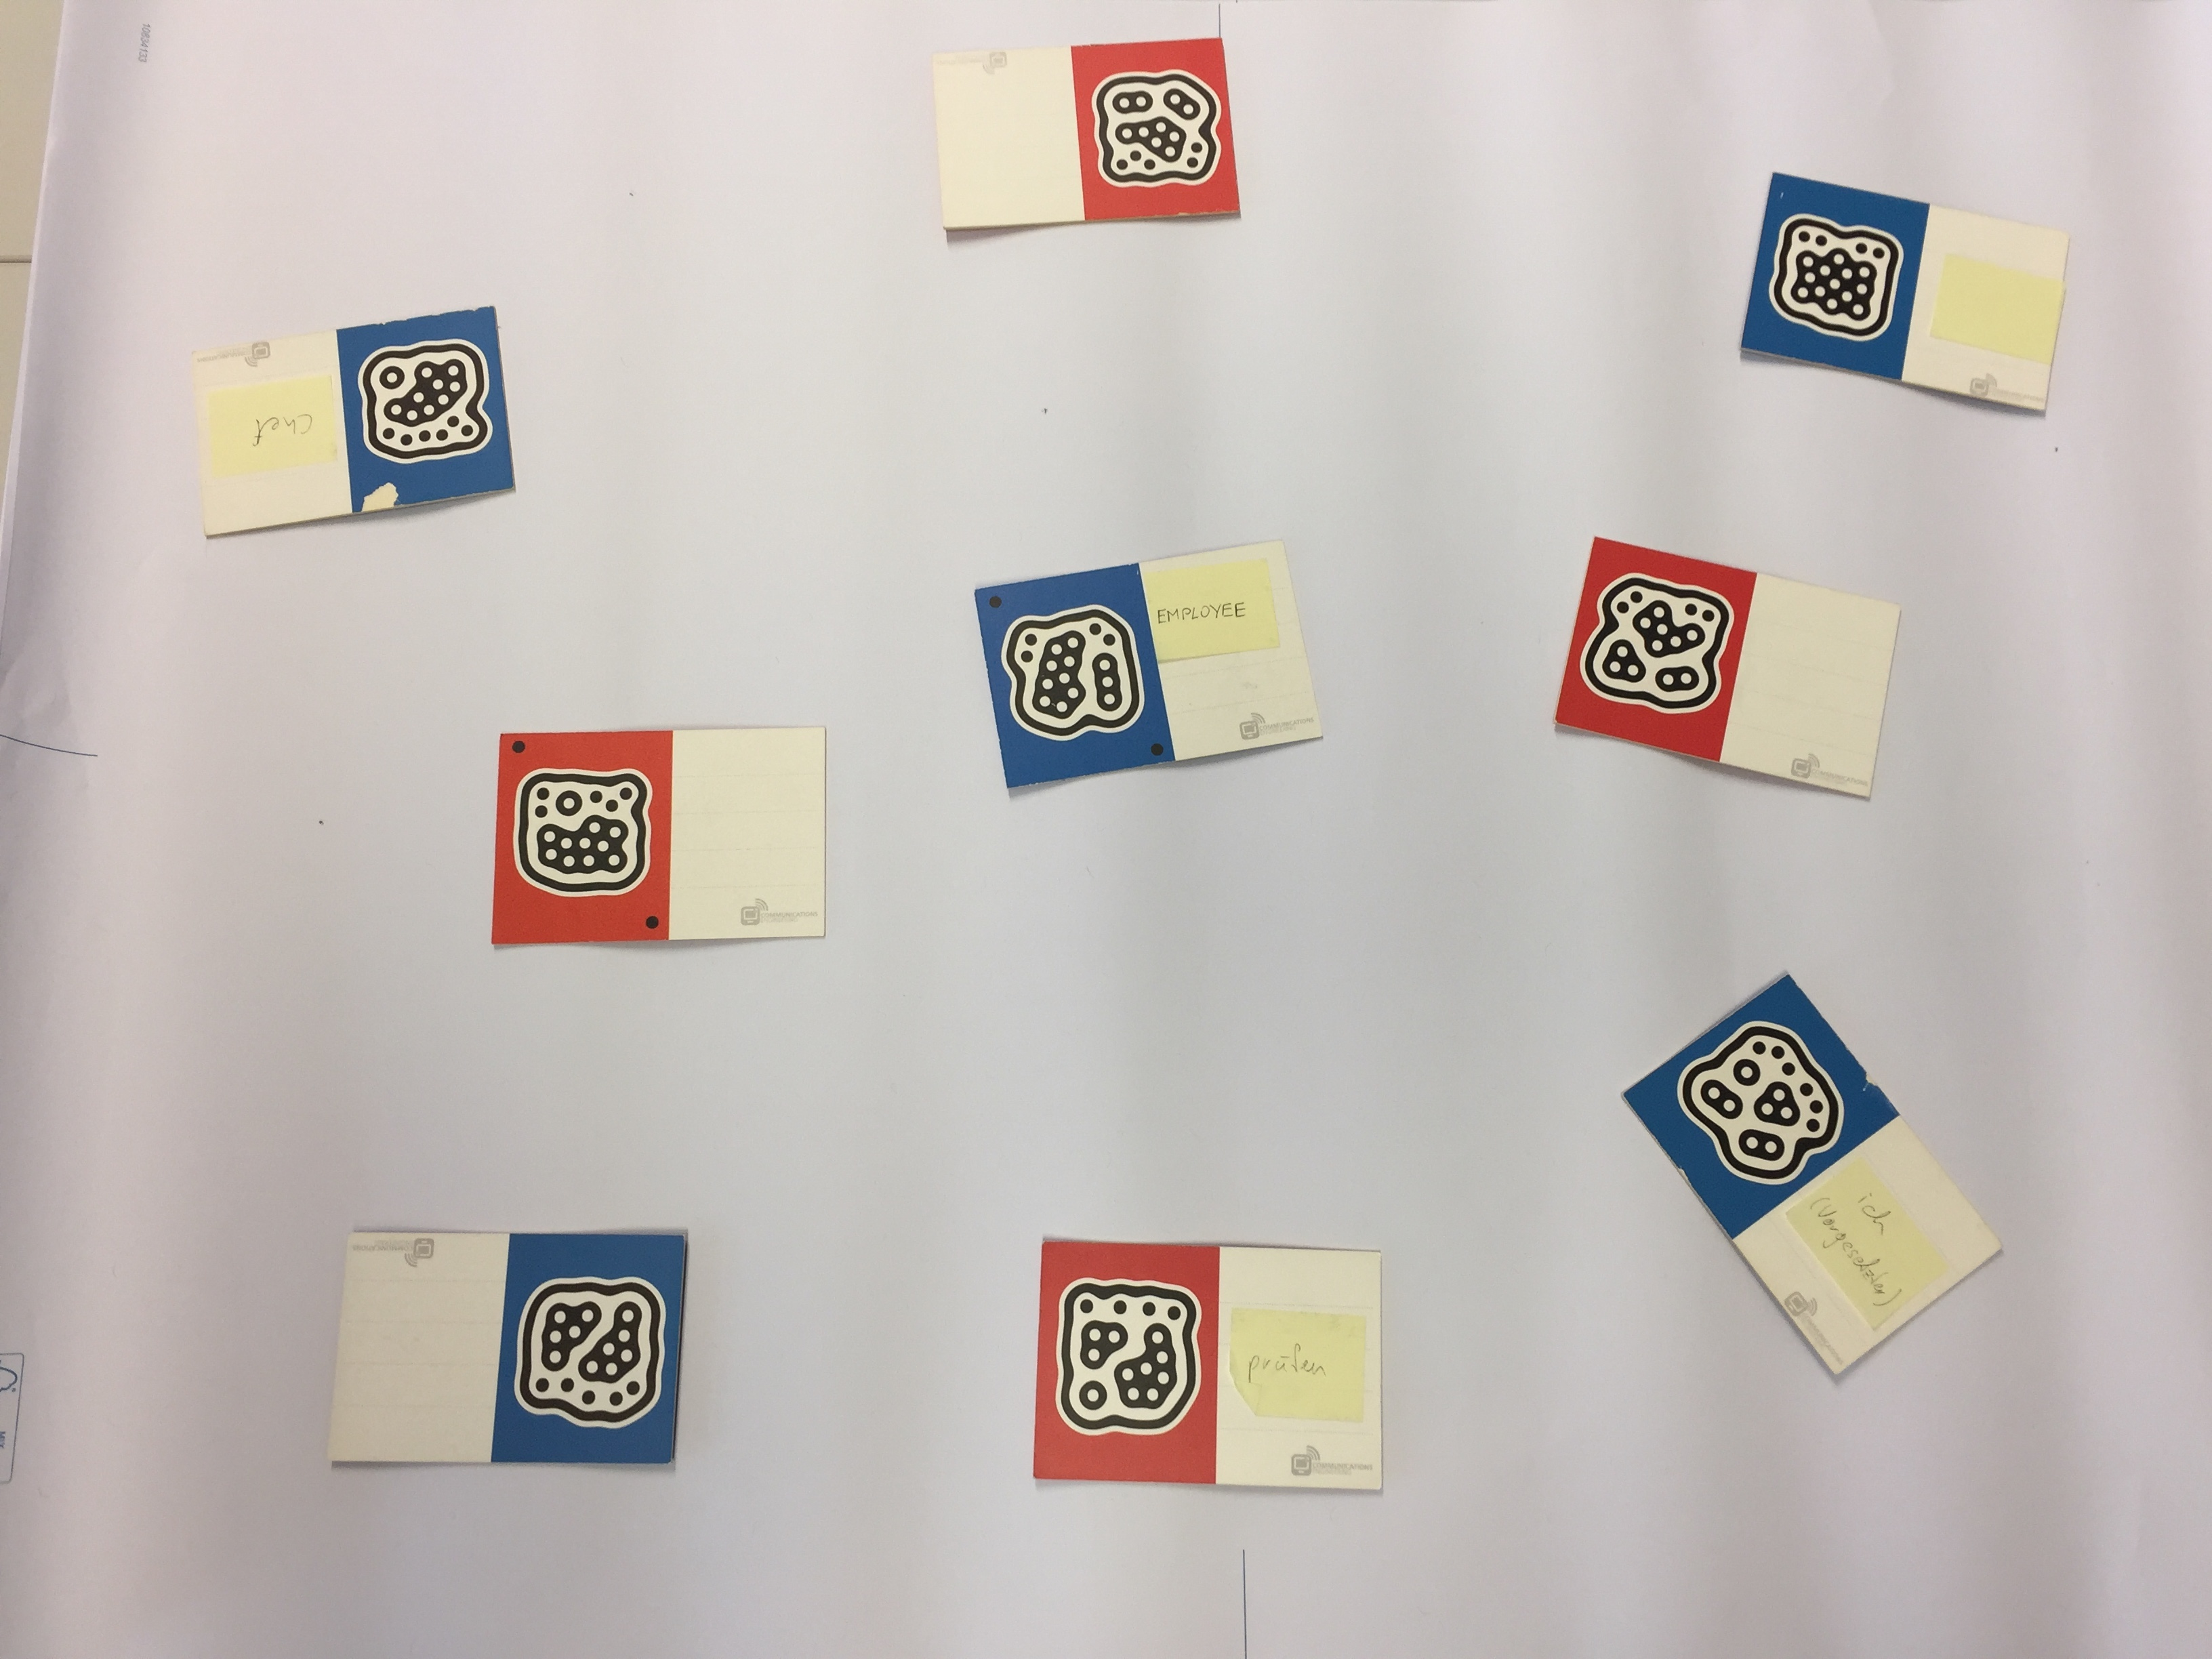
\includegraphics[width=\linewidth]{figures/12.jpg} & Ja & Der Testfall wird als Sternmuster erkannt. \\
		\midrule
		13 & 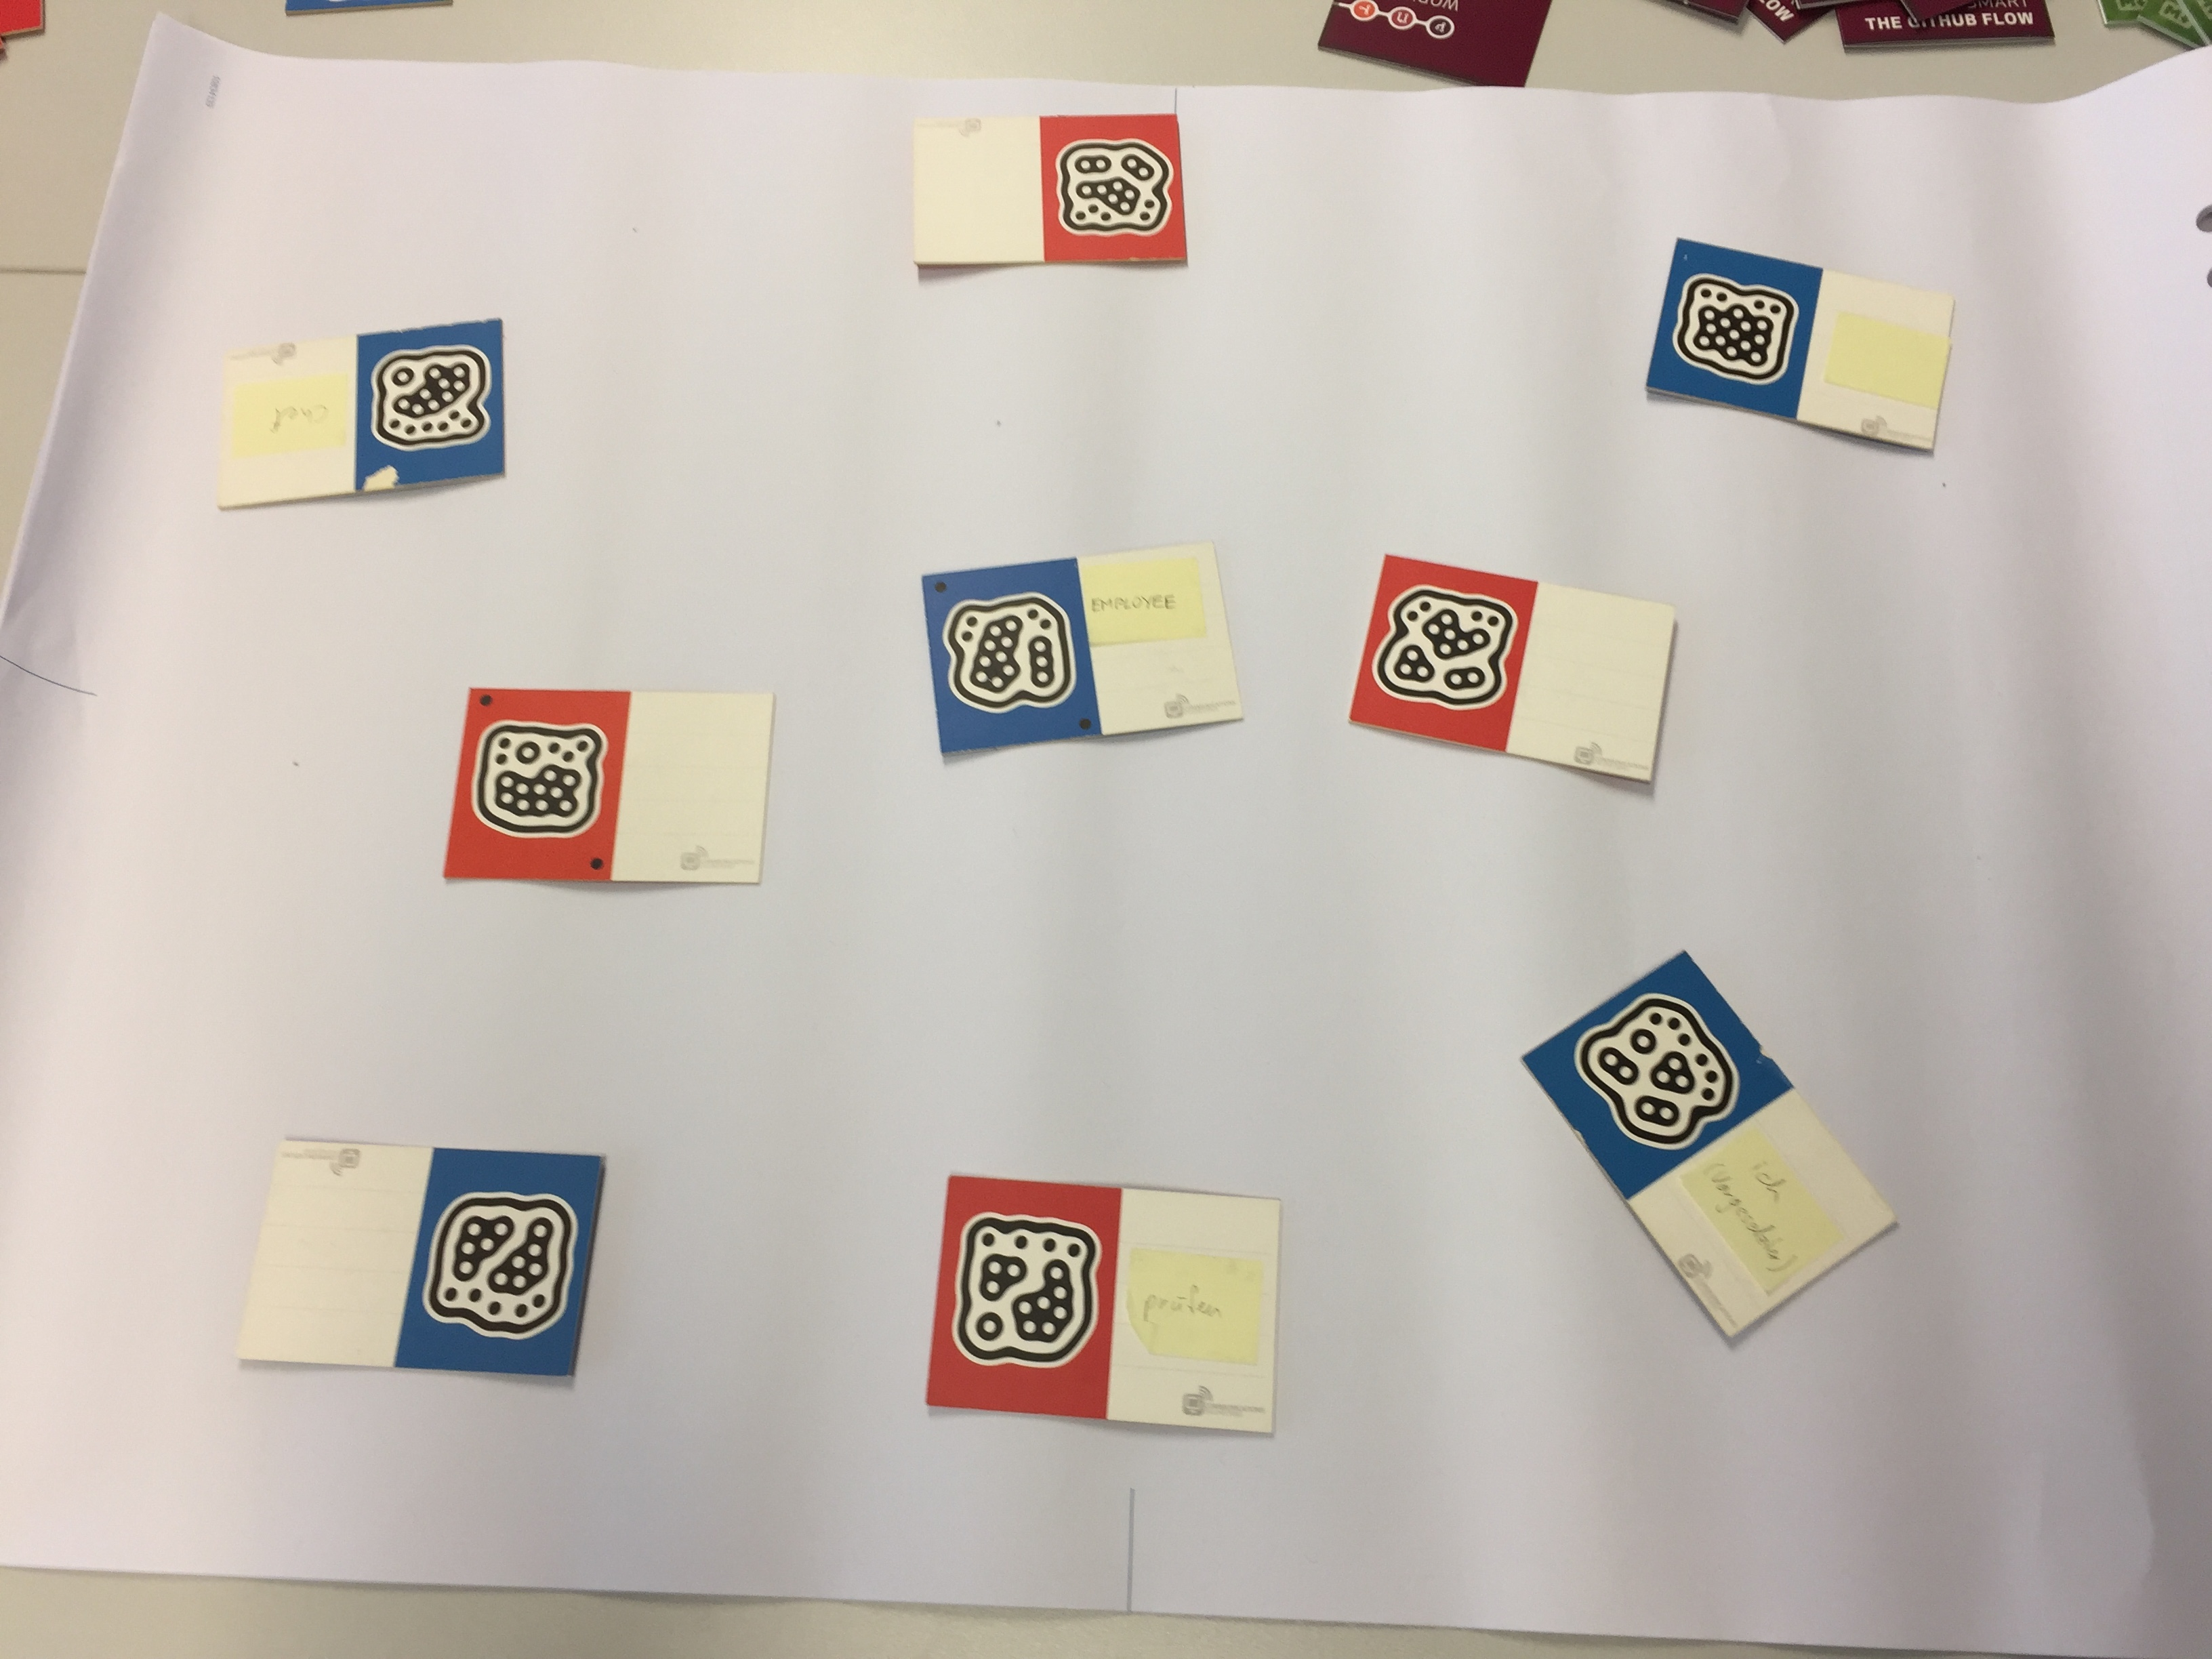
\includegraphics[width=\linewidth]{figures/13.jpg} & Ja & Der Testfall wird als Sternmuster erkannt. \\
		\midrule
		14 & 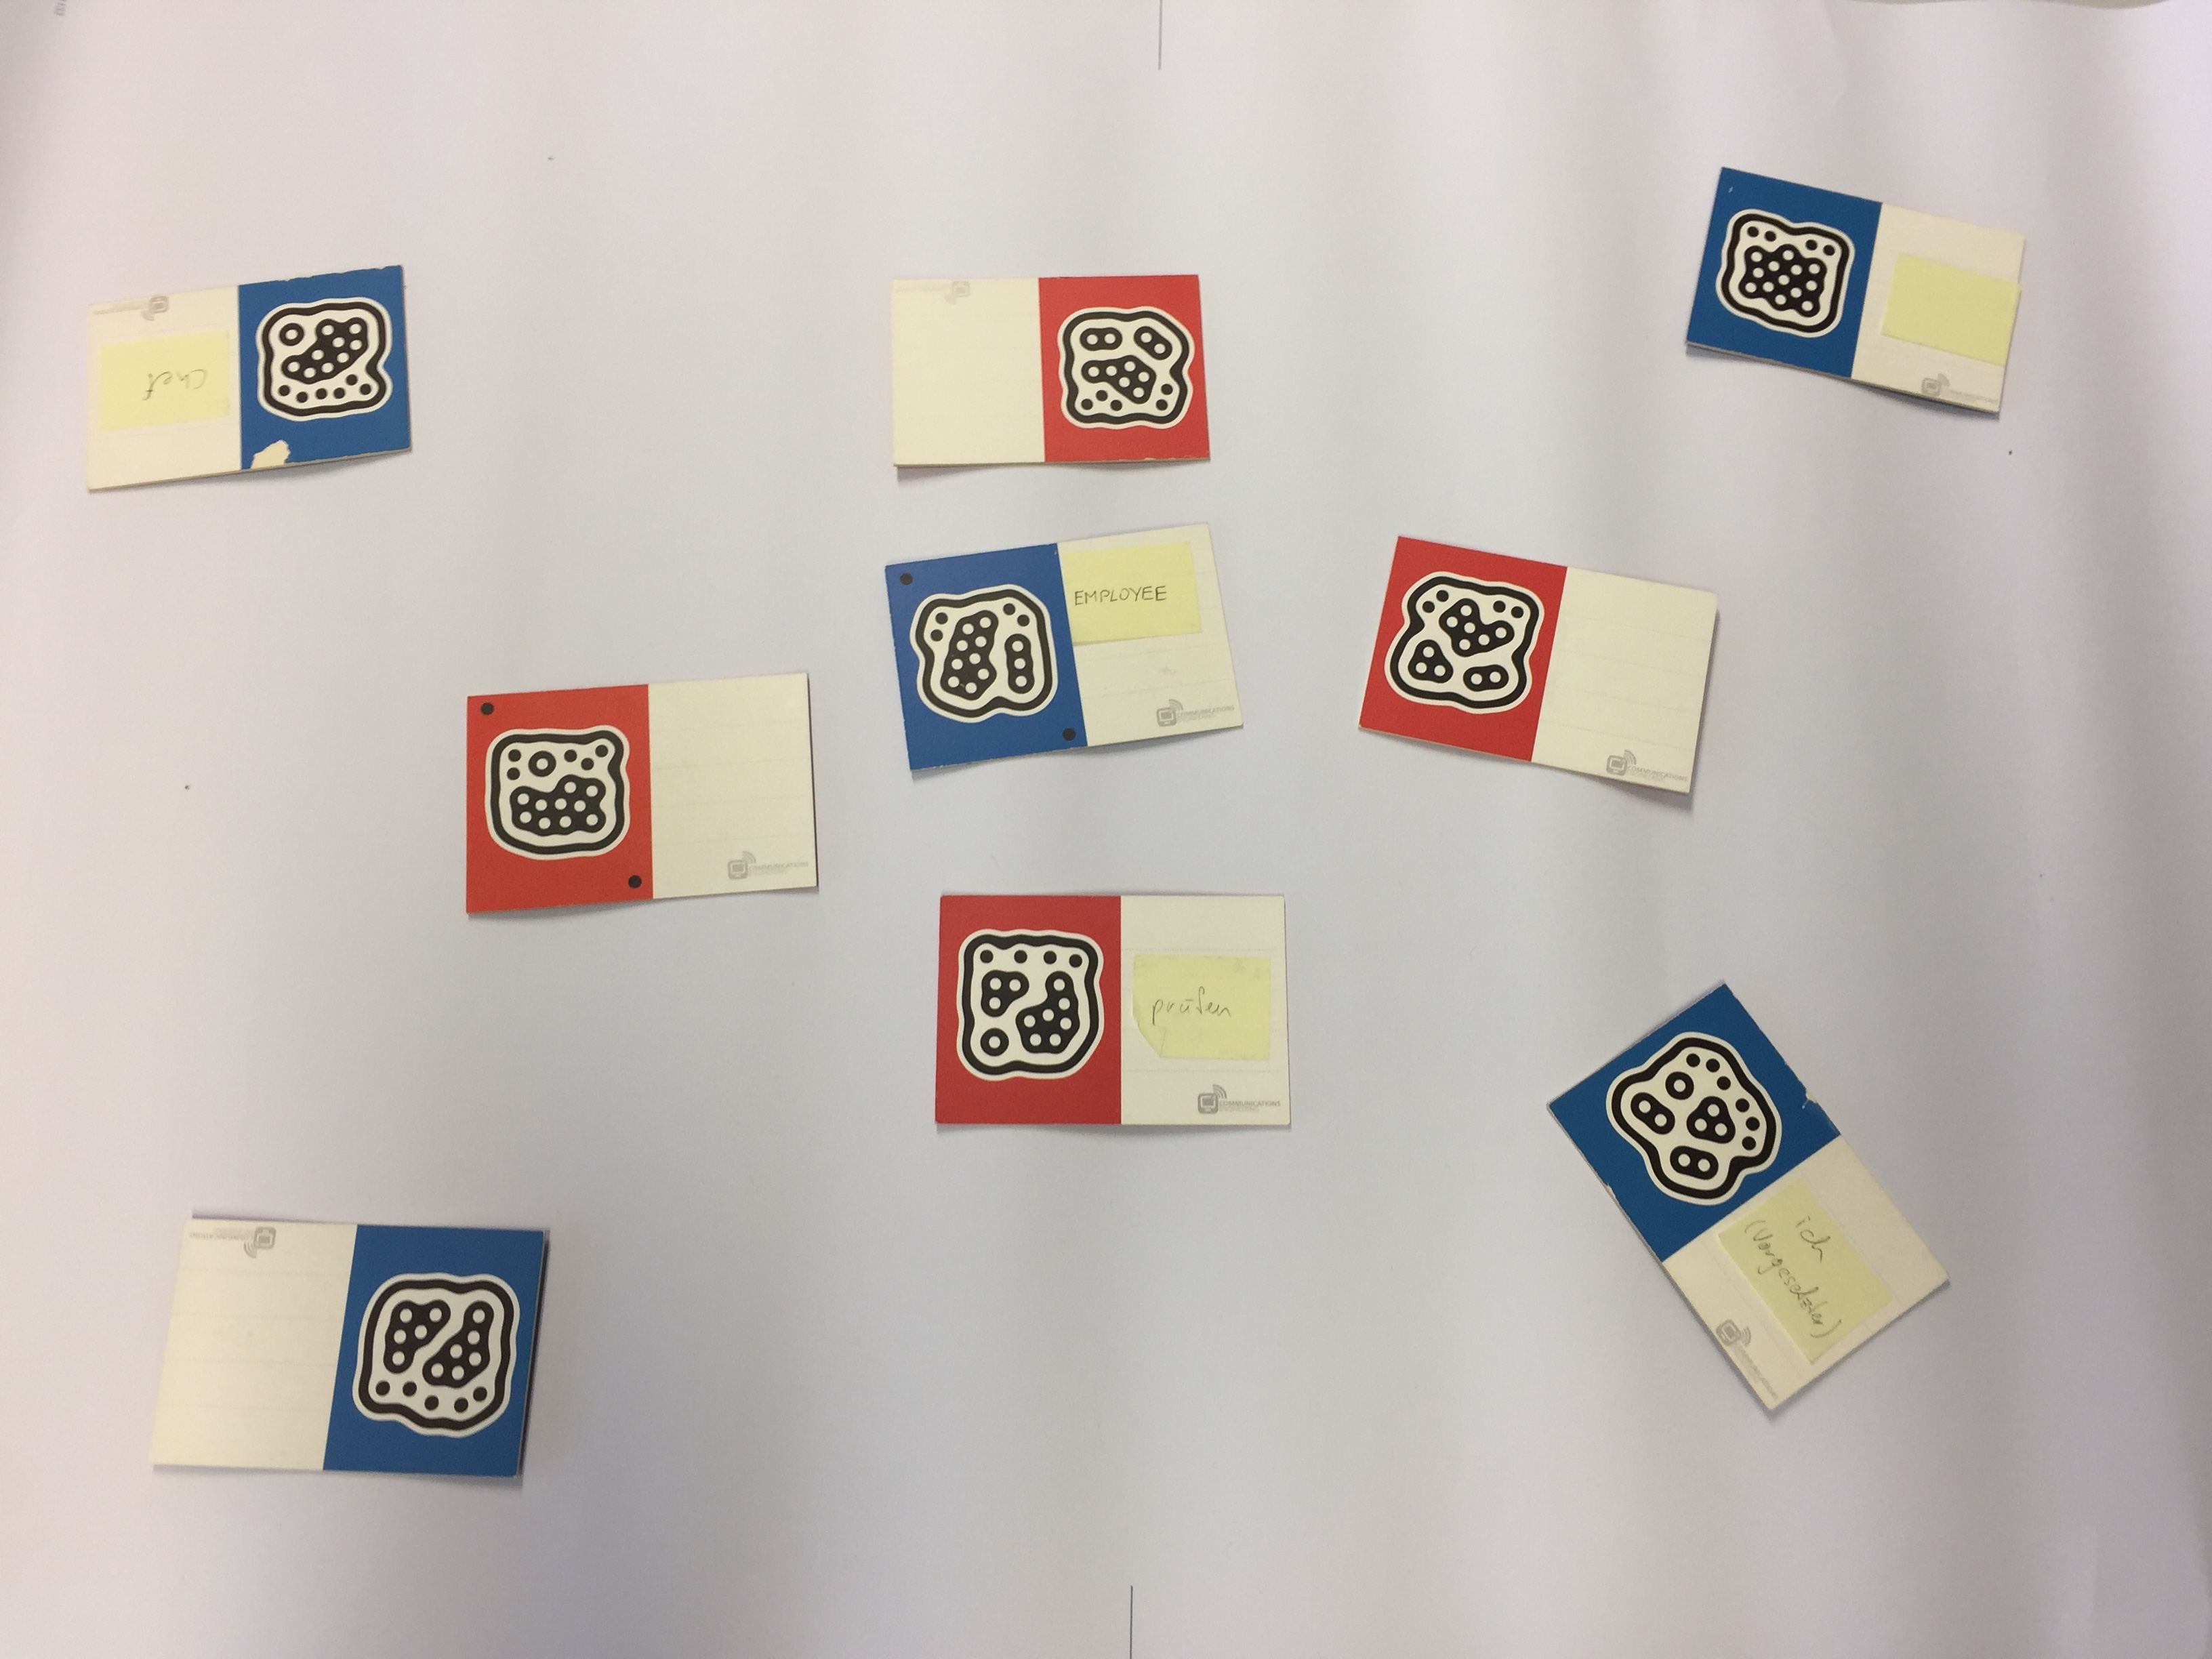
\includegraphics[width=\linewidth]{figures/14.jpg} & Ja & Der Testfall wird als Sternmuster erkannt. \\
		\midrule
		15 & 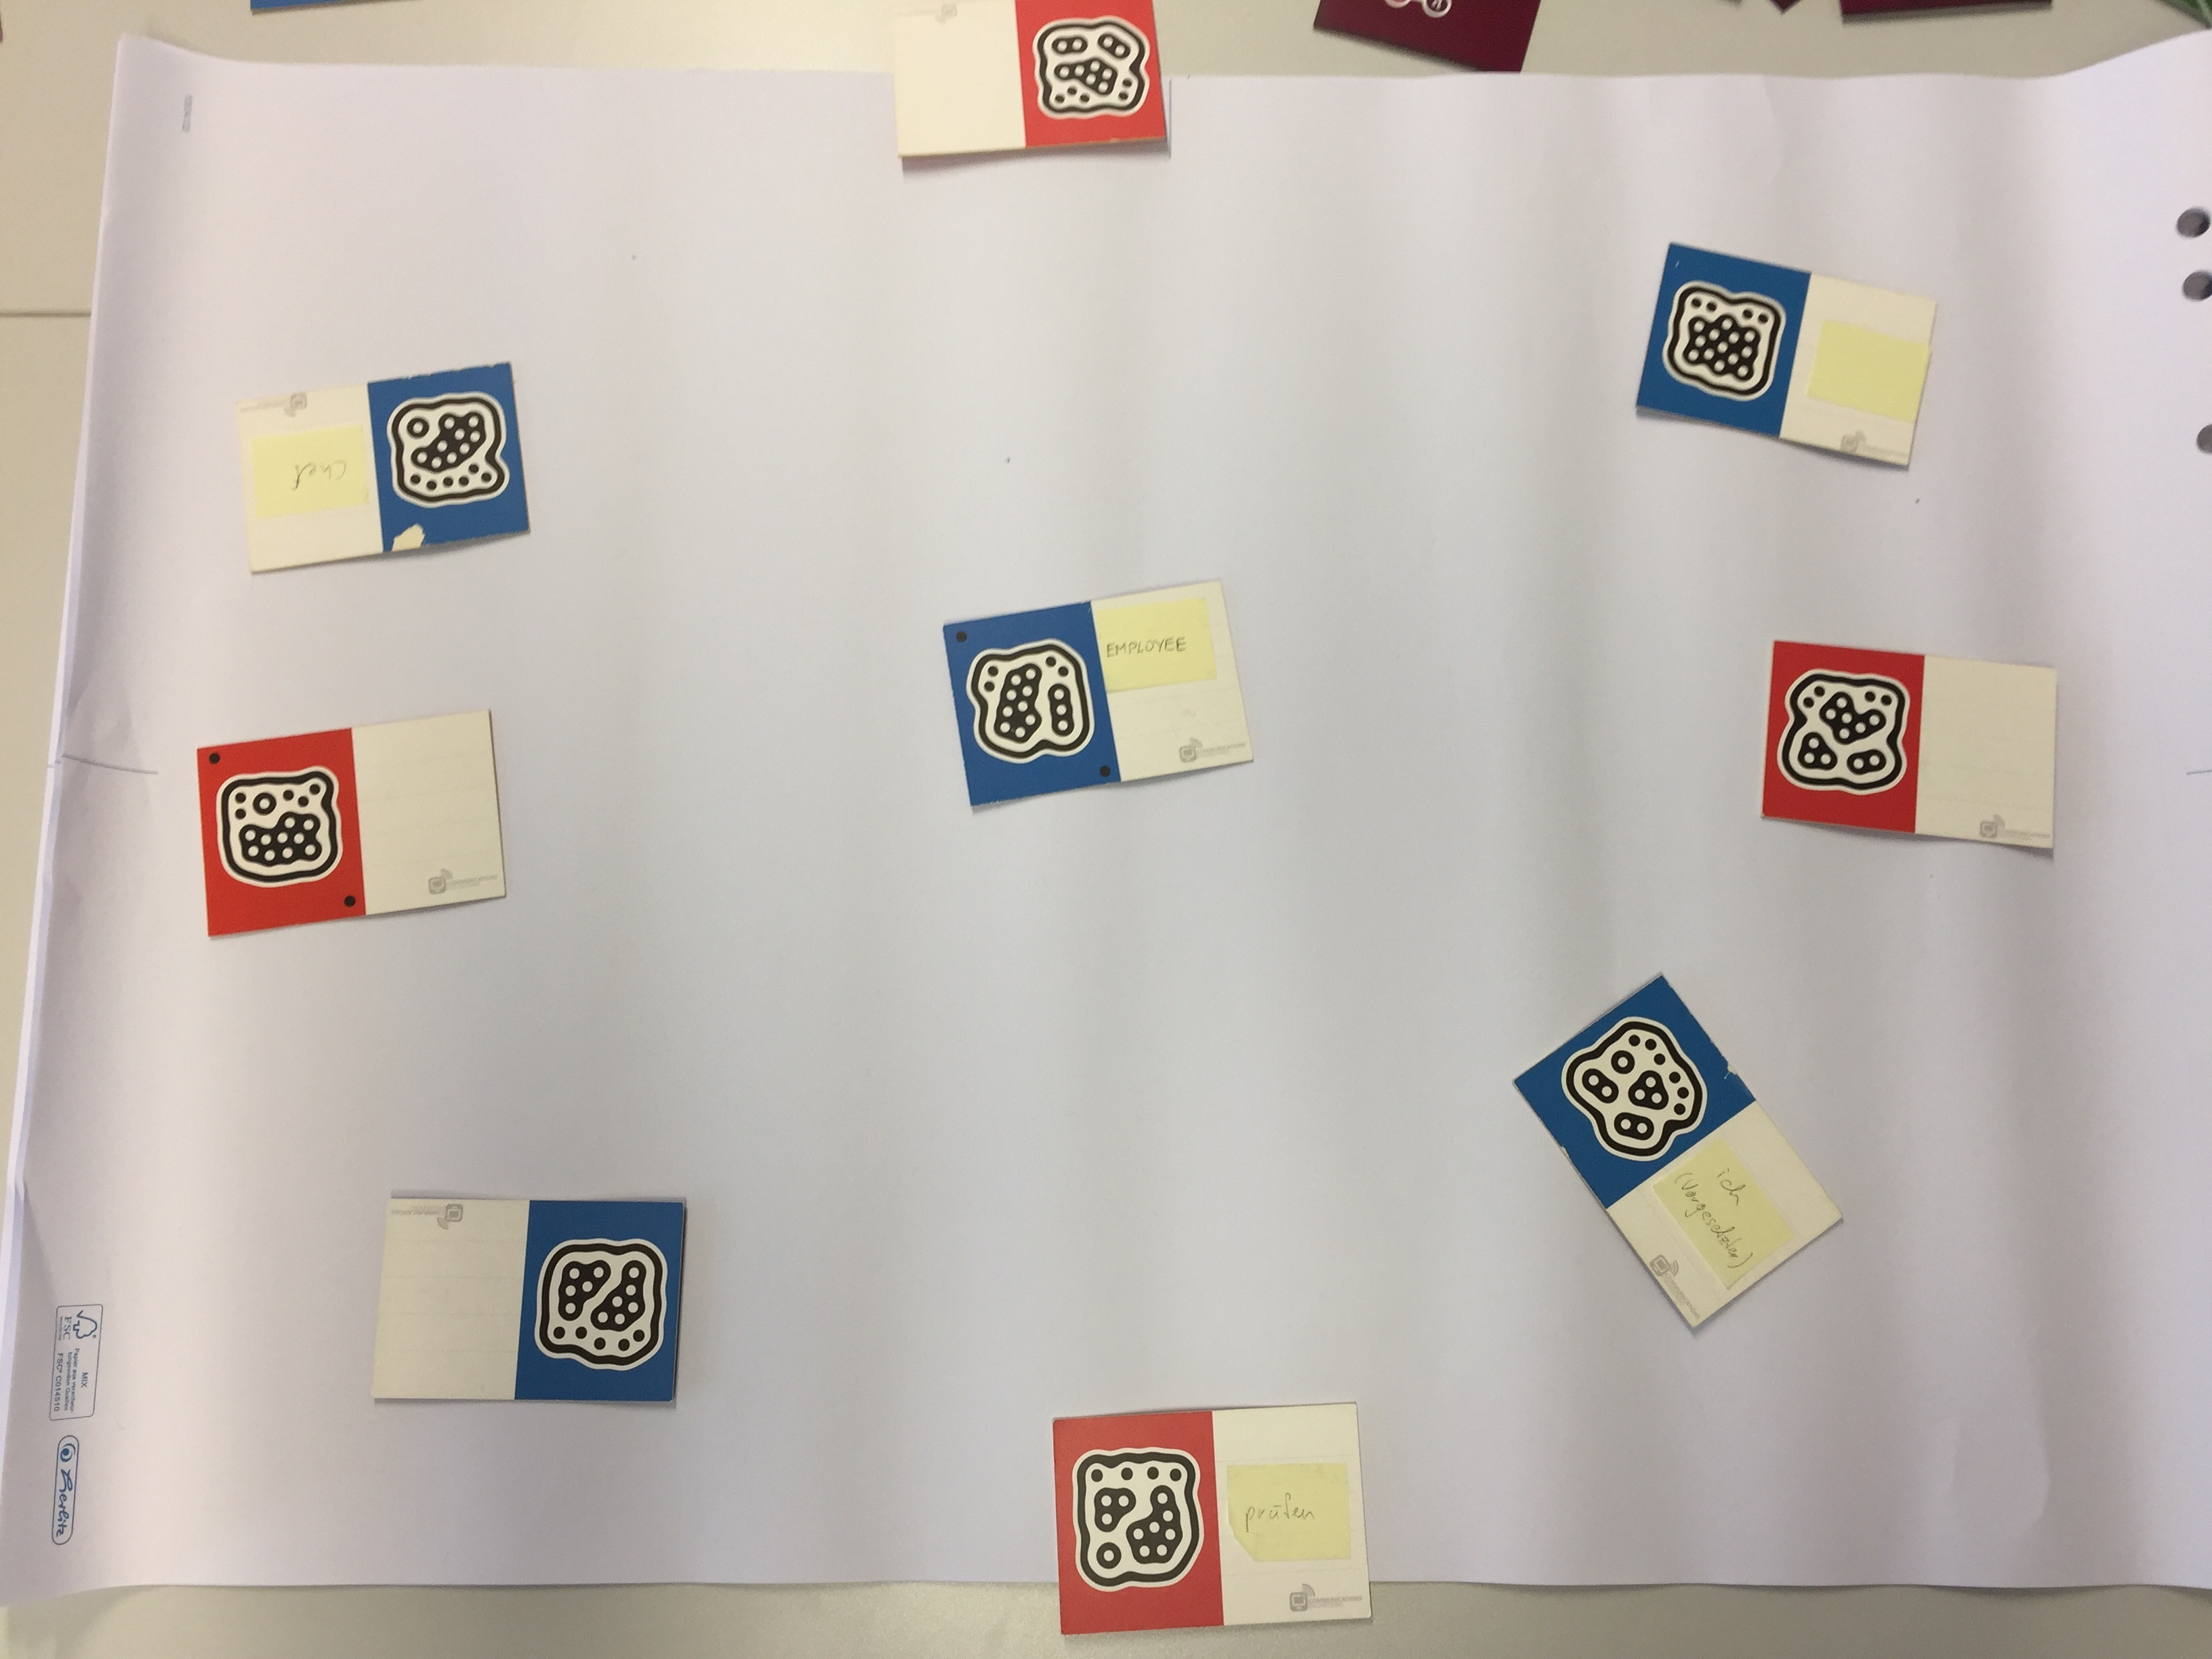
\includegraphics[width=\linewidth]{figures/15.jpg} & Ja & Der Testfall wird als Sternmuster erkannt. \\
		\midrule
		16 & 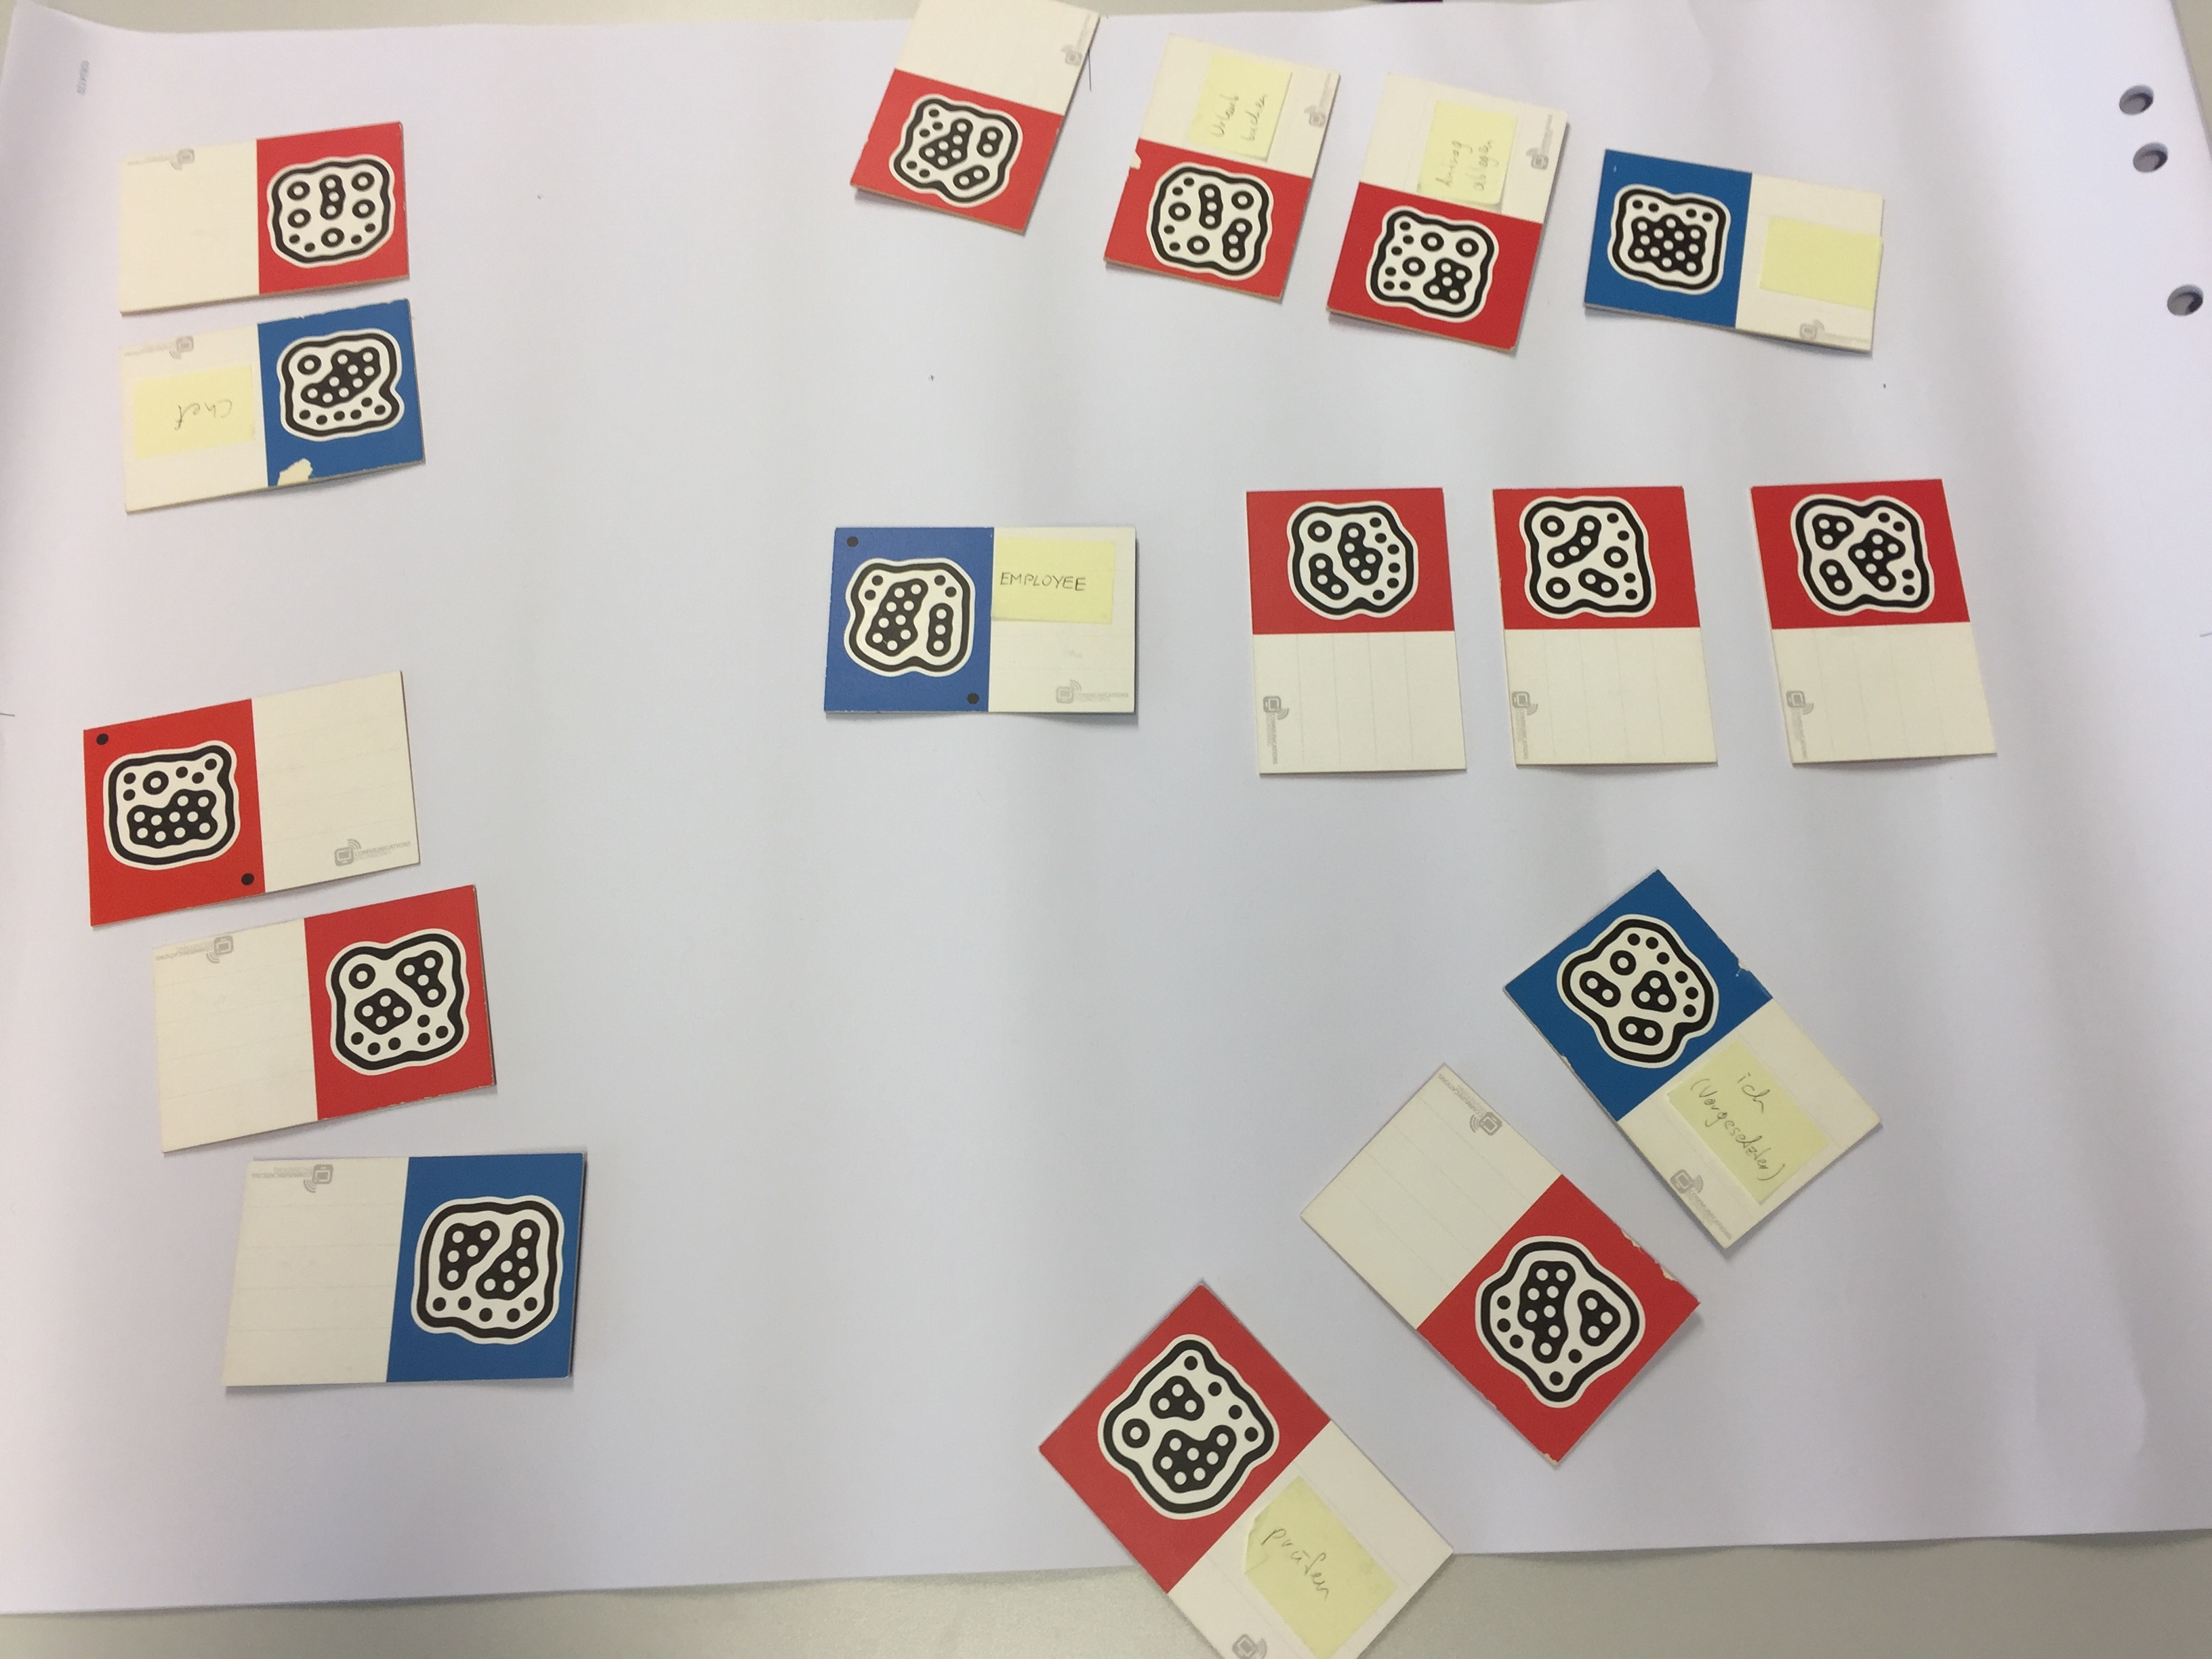
\includegraphics[width=\linewidth]{figures/16.jpg} & Ja & Dieses Beispiel zeigt, dass trotz unterschiedlicher Richtungen die Zuordnungen richtig erkannt werden \\
		\midrule
		17 & 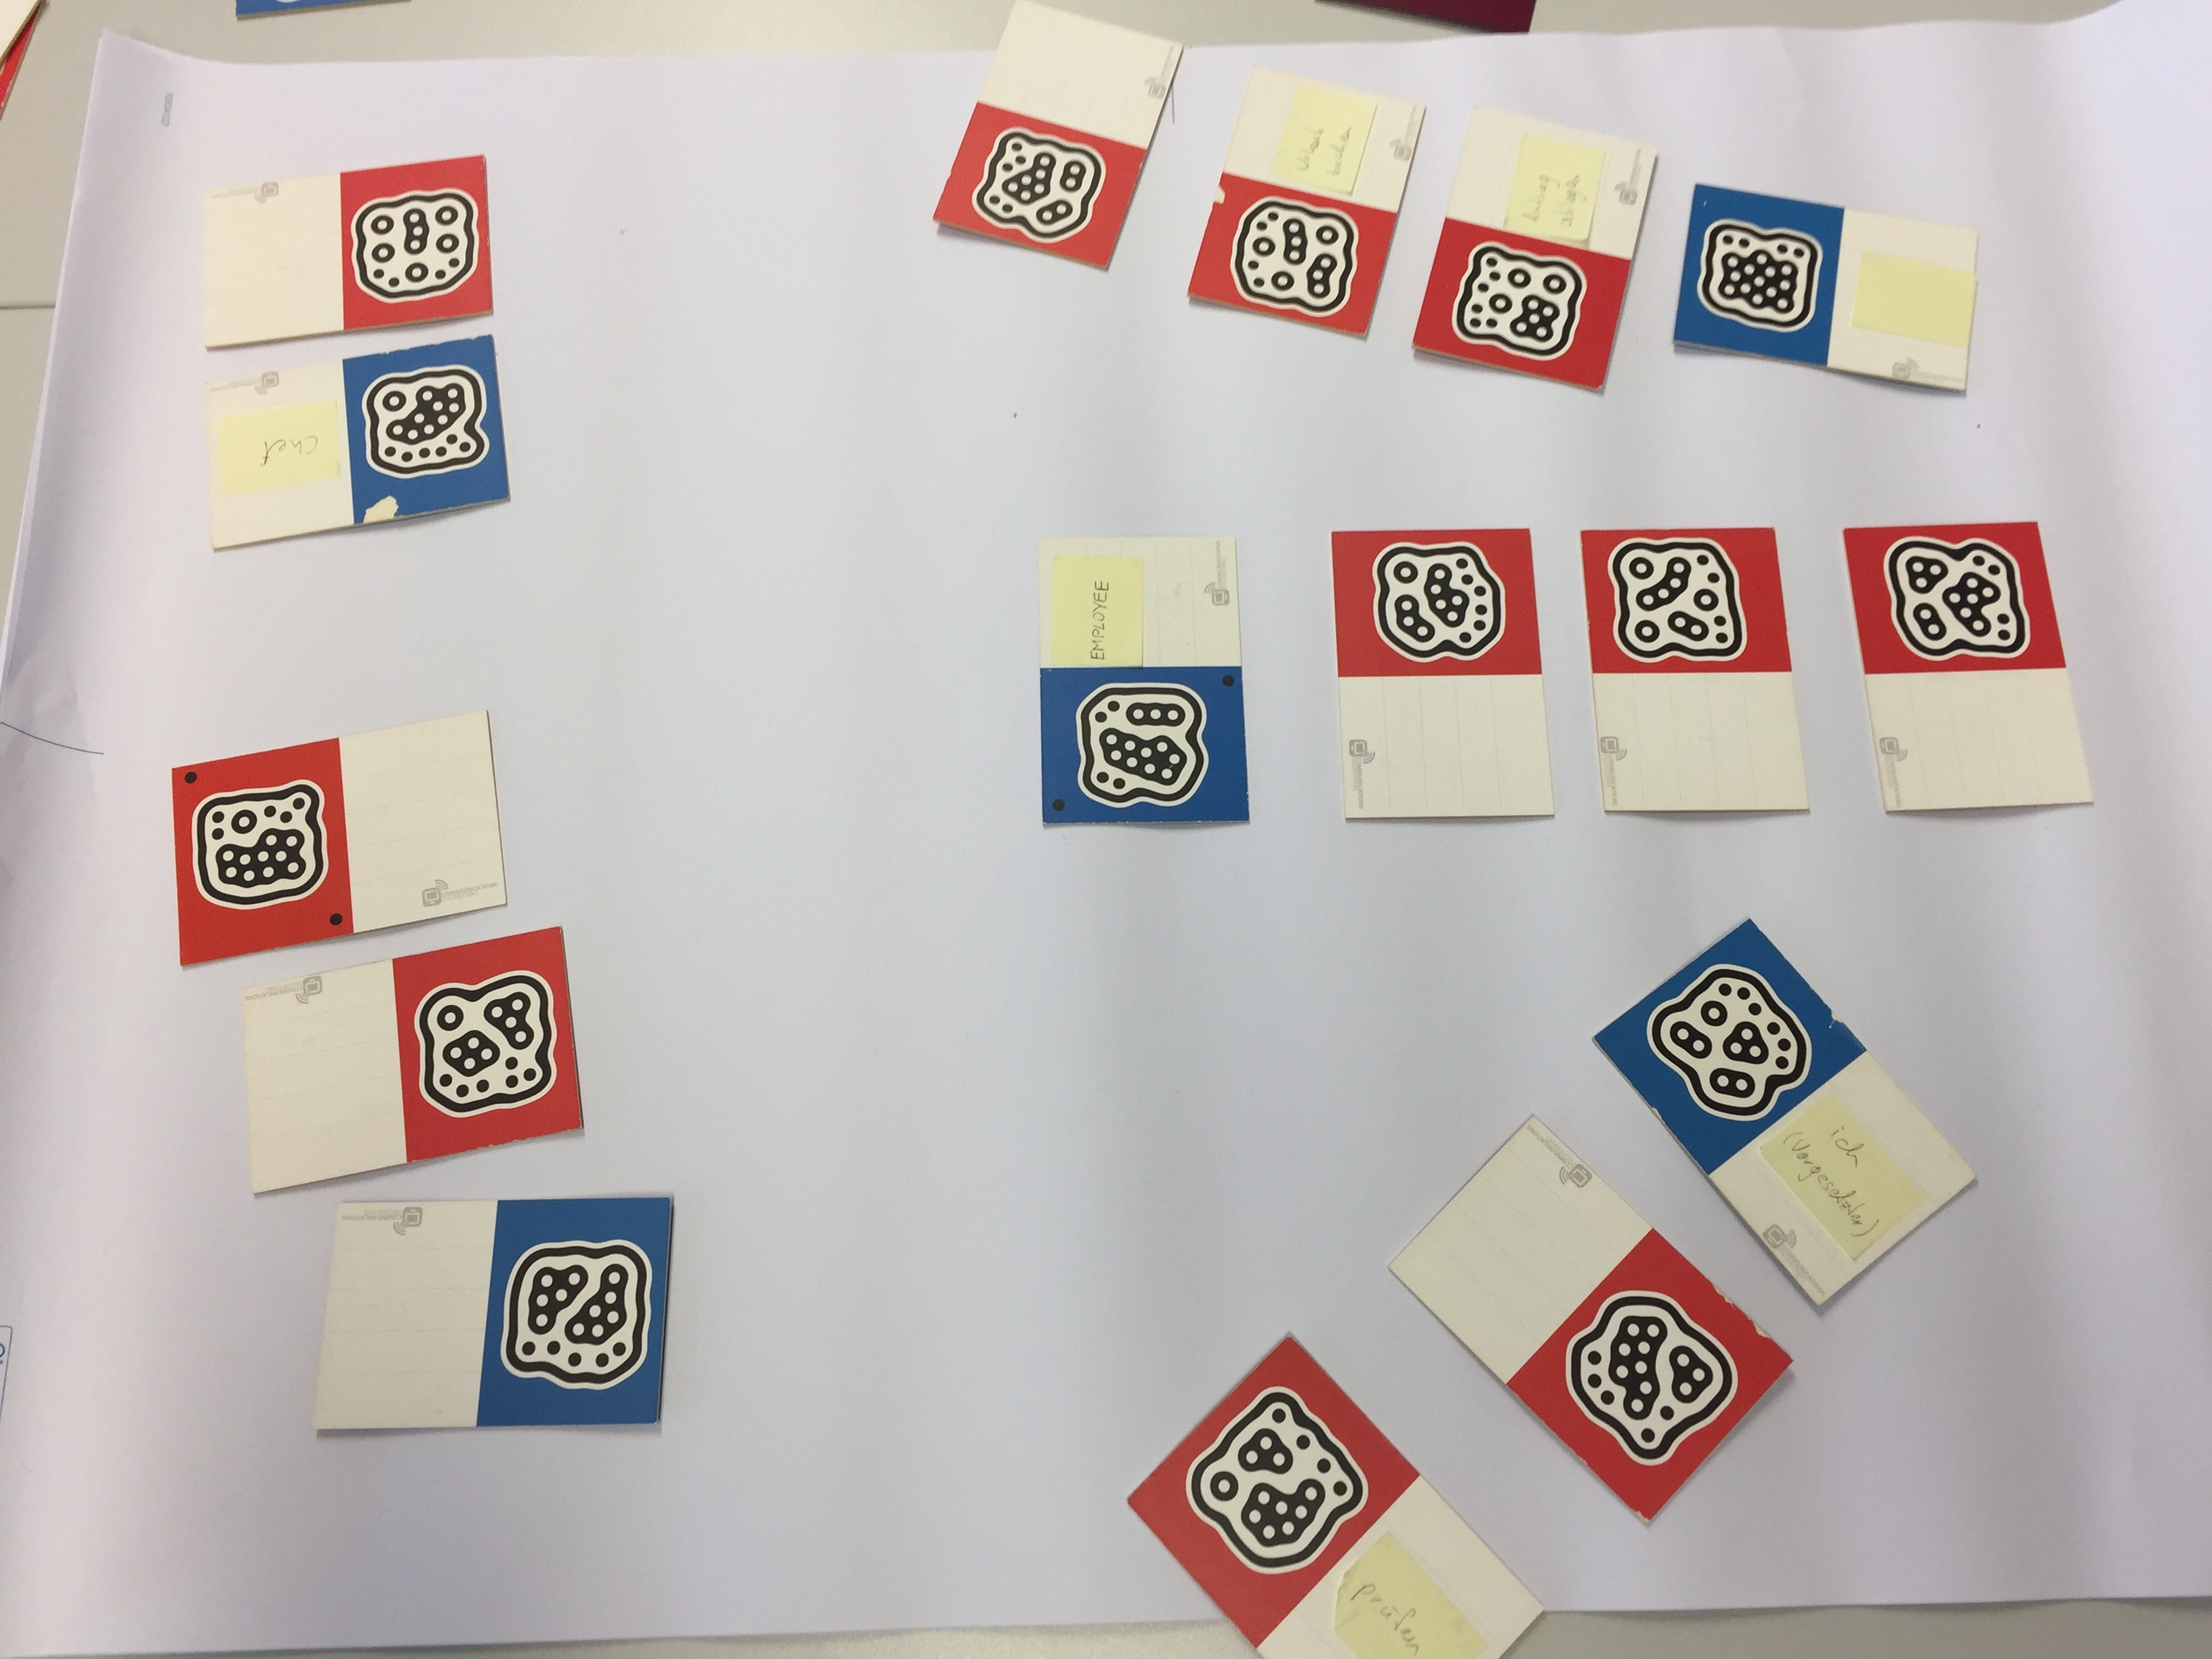
\includegraphics[width=\linewidth]{figures/17.jpg} & Ja & Entspricht in Bezug auf den Algorithmus dem Testfall 16. \\
		\midrule
	\end{longtabu}
\end{center}
}

Die Ergebnisse zeigen, dass der Algorithmus für die vorgegebenen Beispiele fehlerfrei funktioniert. 

% section testergenisse (end)


